\documentclass{report}

\input{latex-temp/preamble.tex}
\input{latex-temp/macros}
\input{latex-temp/letterfonts}

\usepackage[utf8]{inputenc}
\usepackage{fontawesome}
\usepackage{diagbox} % Removed as the package is not found
\usepackage{tikz}
\usepackage{amssymb}
\usepackage{array}
\usepackage{amsmath}
\usepackage{pgfplots}

\pgfplotsset{compat=1.18}
\usepgfplotslibrary{fillbetween}



\newcommand{\dperp}{\mathrel{\bot\!\!\!\bot}}
\renewcommand{\P}{\mathbb{P}}
\newcommand{\p}{p_{(X,Y)}(x,y)}
\renewcommand{\ss}{\mathcal{S}_X\times\mathcal{S}_Y}
\newcommand{\xy}{(X,Y)}


\usetikzlibrary{arrows.meta, positioning}


\setlength{\parindent}{0pt}

\title{\Huge{Probabilità}\\Appunti}
\author{\huge{Giovanni "Qua' Qua' dancer" Palma}\\\huge{e}\\\huge{Alex "Morbidelli WhatsApp" Basta}}
\date{}
\pagenumbering{gobble}

\begin{document}

\maketitle
\newpage% or \cleardoublepage
% \pdfbookmark[<level>]{<title>}{<dest>}
\pdfbookmark[section]{\contentsname}{toc}
\tableofcontents

\pagebreak

\include{paginette/spazi-di-probabilita-discreti}
% \begin{document}
\chapter{Probabilita' Condizionata}

\section{Definizione e motivazioni}

Supponiamo di sapere che un evento di un'esperimento aleatorio si e' avverato. Finora abbiamo visto solo casi in cui gli eventi non si influenzavano (\textit{indipendenti}), ma succede spesso nella realta' che se si sa che un certo evento e' avvenuto, allora questo ci da' informazioni aggiuntive che possono cambiare la probabilita' di altri eventi di cui ancora non sappiamo gli esiti.

Chiamiamo $ B $ l'evento che e' avvenuto e $ A $ un altro evento di cui vogliamo sapere la probabilita'. Prima di avere informazioni su $ B $, la probabilita' di $ A $ era semplicemente $ \mathbb{P}(A) $, ma ora ci poniamo la domanda: "se so che si e' verificato $ B $, come cambia $ \mathbb{P}(A) $?". Denotiamo questa nuova probabilita' con:
\[
  P(A|B)
\]
chiamata la \textit{probabilita' condizionata di  A  dato  B }.

\dfn{Probabilita' Condizionata}{
  Prendo due eventi $ A, B $ su uno spazio di probabilita' $ \left( \Omega, \mathbb{P} \right) $. Definisco \textit{probabilita' condizionata a B di A} la funzione:
  \begin{align*}
    \mathbb{P}(A|B): \powerset(\Omega) &\to [0,1]\\
    A &\mapsto \frac{\mathbb{P}(A \cap B)}{\mathbb{P}(B)}
  \end{align*}
}
E' possibile dimostrare che una certa funzione e' anch'essa una probabilita' (sempre discreta), verifichiamo gli assiomi (fissiamo $ B \subseteq \Omega $ con $ \mathbb{P}(B) > 0 $):
\begin{enumerate}
  \item $ \mathbb{P}(A|B) \in [0,1], \forall A \subseteq \Omega $
  \item $ \mathbb{P}(\Omega|B) = 1 $
  \item $ \sigma-\text{addittivita'} $: $ (A_i)_{i \in \mathbb{N}} $ disgiunti:
    \[
      \mathbb{P}(\bigcup_{i=1}^{\infty} A_i|B) = \sum_{i=1}^{\infty} \mathbb{P}(A_i|B)
    \]
\end{enumerate}
Lasciate al lettore in quanto davvero molto facili, quasi banali. Se non riesci a farle fai schifo.

Vediamo ora, con un esempio, come mai e' proprio questa la definizione utilizzata:
\ex{}{
  \begin{itemize}
  \item 
  Lancio del dado: $ \Omega = \{1,2,3,4,5,6\} $, $ \mathbb{P} $ probabilita' uniforme:

  $ \mathbb{P}(\{\omega\}) = \frac{1}{|\Omega|}, \forall \omega \in \Omega $, ovvero:
  \[
    \mathbb{P}(A) = \frac{\text{casi favorevoli in }A}{\text{casi possibili}}
  \]
  $ A = \text{"esce un numero maggiore di 3"} = \{3,4,5,6\} $ e $ B = \{\text{"esce un numero pari"}\} = \{2,4,6\} $, domanda: quanto vale $ \mathbb{P}(A|B) $?

  $ P(A) = \frac{4}{6} $ come abbiamo gia visto.

  Ora abbiamo un'informazione in piu': sappiamo che $ B $ si e' avverato. Questo significa che si restringe l'insieme di valori che possono essere usciti al lancio del dado. ATTENZIONE! cio' non vuol dire che cambia lo spazio campionario perche' l'esperimento e' lo stesso, ma cambiano i \textit{veri} casi favorevoli e i \textit{veri} casi possibili:
  \[
    P(A|B) = \frac{\text{"veri casi favorevoli di A"}}{\text{veri casi possibili}} = \frac{|A \cap B|}{|B|} = \frac{2}{3}
  \]
  \item
  Vediamo anche cosa accade quando la probabilita' non e' uniforme, come con un dado a 4 facce truccato: 

  $ \Omega = \{1,2,3,4\} $, $ \mathbb{P}(4)=\frac{1}{15}, \mathbb{P}(3)=\frac{2}{15}, \mathbb{P}(2)=\frac{4}{15}, \mathbb{P}(1)=\frac{8}{15} $

  $ A = \{3,4\}, B = \{2,4\} $
  \[
    \mathbb{P}(A|B) = \frac{\text{"probabilita' dei veri casi favorevoli di A"}}{\text{probabilita' dei veri casi possibili}} = \frac{\mathbb{P}(A \cap B)}{\mathbb{P}(B)}
  \]
  \end{itemize}

}

\nt{
  Se $ \mathbb{P} $ e' la probabilita' uniforme allora:
  \[
    \mathbb{P}(A|B) = \frac{\mathbb{P}(A \cap B)}{\mathbb{P}(B)} = \frac{\frac{|A \cap B|}{|\Omega|}}{\frac{|B|}{|\Omega|}} = \frac{|A \cap B|}{|B|}
  \]
}

\nt{
  B e' fissato nella definizione di propbabilita' condizionata, ovvero:
  \[
    \mathbb{P}(A|B) \neq \mathbb{P}(B|A)
  \]
  Quindi il ruolo di $ A $ e $ B $ e' completamente diverso
}

\nt{
  Se $ B = \Omega $, allora $ \mathbb{P}(A|B) = \mathbb{P}(A) $ dato che la conoscenza del fatto che si e' avverato $ \Omega $ e' ovvio e non ci cambia.

  Se $ A = \Omega $, allora $ \mathbb{P}(\Omega | B) = 1 $ (per proprieta', dato che e' sempre una probabilita')
}

\section{Regola della catena}

La probabilita' condizionata in genere e' nota e si usa per calcolare la probabilita' dell'intersezione:
  \[
    \mathbb{P}(A \cap B) = \mathbb{P}(A|B) \cdot \mathbb{P}(B)
  \]
Questa formula e' detta \textit{regola della catena} e vale in generale con $ n $ eventi:

\mprop{Regola della catena (generalizzata)}{
  $ (A_i)_{i = 1,...,n}, \mathbb{P}(A_1 \cap ... \cap A_{n-1}) > 0 $, allora:
  \[
    \mathbb{P}(A_1 \cap ... \cap A_n) = \mathbb{P}(A_1)\mathbb{P}(A_2|A_1)\mathbb{P}(A_3|A_1 \cap A_2) ... \mathbb{P}(A_n| A_1 \cap ... A_{n-1})
  \]
}
\nt{

  La condizione funziona grazie alla monotonia, dato che $ 0 < \mathbb{P}(A_1 \cap ... \cap A_{n-1}) \leq \mathbb{P}(A_1 \cap ... \cap A_j), 1 \leq j \leq n-1 $ quindi siamo certi che l'intersezione degli eventi che sono avvenuti e' maggiore di 0.
}
\pf{}{
  $ P(A_1) \frac{P(A_1 \cap A_2)}{P(A_1)}...\frac{P(A_1 \cap ... \cap A_n)}{P(A_1 \cap ... \cap A_{n-1})}= P(A_1 \cap ... \cap A_n) $
} 
TODO: migliora un po

\ex{}{
Un’urna contiene tre palline bianche, due palline nere e una pallina rossa.
Si eseguono tre estrazioni senza reimmissione.
Qual `e la probabilit`a di estrarre nell’ordine una bianca, una rossa e una nera?

  Sono interessato solo ad alcuni eventi, quindi non c'e' bisogno di descrivere l'intero esperimento aleatorio. Per prima cosa definisco l'evento:
  \[
  A = \text{"estrarre in ordine una bianca, una rossa e una nera"}
  \]
  Voglio trovare $ P(A) $. Notiamo che dobbiamo determinare tre sottoesperimenti in relazione (dato che non c'e' reimissione). Quindi dopo ogni sottoesperimento cambia la composizione dell'urna, e sappiamo come calcolare la probabilita' condizionata:
  \[
  B_i = \text{"estraggo una pallina bianca all' i-esimo turno"}
  \]
  \[
  R_i = \text{"estraggo una pallina rossa all' i-esimo turno"}
  \]
  \[
  N_i = \text{"estraggo una pallina nera all' i-esimo turno"}
  \]
  Esistono tre famiglie di eventi: $ (B_i)_{i = 1,...,k}, (R_i)_{i = 1,...,k}, (N_i)_{i = 1,...,k} $ dove $ i $ indica il turno al quale viene estratta la pallina. Quindi possiamo scrivere $ A $ come relazione fra sottoeventi:
  \[
  A = B_1 \cap R_2 N_3
  \]
  Quindi:
  \[
    P(A) = P(B_1 \cap R_2 \cap N_3) = P(B_1)P(R_2 | B_1)P(N_3 | B_1 \cap R_2)
  \]
  Solo ora possiamo passare ai valori numerici. Dato che gli esiti sono equiprobabili e lo spazio campionario e' finito, la probabilita' e' uniforme:
  \[
    P(B_1) = \frac{1}{2}, P(R_2) = \frac{1}{5}, P(N_3) = \frac{1}{2}
  \]
  \[
    P(A) = \frac{1}{20}
  \]
}

Per esperimenti formati da sottoesperimenti di cui conosco le probabilita' condizionate, e' possible rappresentare ogni evento come un nodo:
\[
\Omega = \text{primo nodo}
\]
e ogni probabilita' come un ramo che partiziona il nodo (tanti rami quanti gli insiemi della partizione) che rappresenta poi un altro evento (condizionato dalla seconda in poi).

\begin{center}
  \includegraphics[width=0.5\textwidth]{img/2025-02-28-13-59-32.png}
\end{center}

La regola della catena la leggo sul diagramma ad albero:

percorso: $ \Omega \to B_1 \to R_2 \to N_3 $ ha probabilita' $ P(B_1 \cap R_2 \cap N_3) $ che si calcola facendo il prodotto delle probabilita' dei relativi rami che si usano nel percorso.

E' uno strumento utile per convincerci che stiamo usando le formule guiste, ma non le sostituisce e puo' diventare laborioso per problemi complessi.

\ex{}{
Ci sono due urne: la prima contiene due palline rosse e una bianca; la
seconda contiene tre palline rosse e due bianche. Si lancia una moneta: se esce testa si
estrae una pallina dalla prima urna, se esce croce si estrae una pallina dalla seconda urna.
Qual `e la probabilit`a che l’esito del lancio della moneta sia testa e la pallina estratta sia
bianca?

  2 sottoesperimenti:
  \begin{itemize}
  \item lancio della moneta
  \item estrazione da un'urna
  \end{itemize}

  Nota che i sottoesperimenti sono indipendenti dall'esito di altri esperimenti. Sono gli esiti, ovvero i risultati, che possono dipendere dagli esiti di altri esperimenti.

  \[
  A = \text{"esce testa ed estraggo una pallina bianca"}
  \]
  Devo esprimere A con eventi che 
  \[
  T = \text{"esce testa"}
  \]
  \[
  U = \text{estraggo una pallina bianca}
  \]
  Disegna lo zio pera di diagramma che non mi metto a fare, se @GiovanniPalma vuole puo' farlo
  \[
    A = T \cap U, \quad P(A) = P(T)P(U|T)
  \]
}

\section{Indipendenza di eventi}

E' possibile che sapere che un evento $ B $ e' avvenuto non altera la probabilita' di un altro evento $ A $. Possiamo esprimere questa relazione in modo matematico cosi':
\[
  \mathbb{P}(A|B) = \mathbb{P}(A)
\]
Utilizzando la definizione di probabilita' condizionata, possiamo usare un'identita' equivalente che useremo come definizione:
\dfn{Eventi indipendenti}{
  Due eventi $ A, B $ si dicono indipendenti se:
  \begin{equation}
    \mathbb{P}(A \cap B) = \mathbb{P}(A) \cdot \mathbb{P}(B)
  \end{equation}
  

  E viene denatato $A \dperp B$
}

Usiamo questa definizione dato che e' esplicitamente simmetrica, ovvero se A e indipendente a B allora vale anche il contrario:
\[
A \dperp B \iff B \dperp A
\]
ed e' definita (e banalmente vera) anche quando $ \mathbb{P}(A)=0 $ o $ \mathbb{P}(B)=0 $. In particolare si noti il seguente teorema:
\thm{Teorema della simmetria tra eventi indipendenti}{ \label{thm:simmetria_indipendenza}
  Sia $\mathbb{P}(B)>0$ allora:
  \[
    A \dperp B \iff \mathbb{P}(A|B) = \mathbb{P}(A)
  \]
  Dall'altro lato, sia $\mathbb{P}(A)>0$ allora:
  \[
    A \dperp B \iff \mathbb{P}(B|A) = \mathbb{P}(B)
  \]
}

\pf{Dimostrazione}{
  Verrà fornita solo la dimostrazione del primo punto, la seconda parte è analoga.

  Assumo $\mathbb{P}(B)>0$, si ha:
  \begin{itemize}
    \item $ A \dperp B \implies \mathbb{P}(A|B) = \mathbb{P}(A) $:
      \[
        \mathbb{P}(A|B) = \frac{\mathbb{P}(A \cap B)}{\mathbb{P}(B)} = \frac{\mathbb{P}(A) \cdot \mathbb{P}(B)}{\mathbb{P}(B)} = \mathbb{P}(A)
      \]
    \item $ \mathbb{P}(A|B) = \mathbb{P}(A) \implies A \dperp B $:
      \[
        \mathbb{P}(A \cap B) = \mathbb{P}(A|B) \cdot \mathbb{P}(B) = \mathbb{P}(A) \cdot \mathbb{P}(B)
      \]
  \end{itemize}
}

\nt{
  Si noti che se $\mathbb{P}(A)>0$ e $\mathbb{P}(B)>0$ allora, le tre uguaglianze seguenti sono equivalenti:
  \[
    \mathbb{P}(A\cap B) = \mathbb{P}(A) \cdot \mathbb{P}(B) \iff \mathbb{P}(A|B) = \mathbb{P}(A) \iff \mathbb{P}(B|A) = \mathbb{P}(B)
  \]
}

\nt{
  \begin{itemize}
  \item L'indipendenza e' diversa dalla disgiunzione:
  \[
  A \indip B \neq A \cap B = \emptyset
  \]
  infatti sono relazioni ortogonali:
  \[
    A \indip B \land A \cap B = \emptyset \iff \mathbb{P}(A)\mathbb{P}(B) = 0 \iff \mathbb{P}(A) = 0 \lor \mathbb{P}(B) = 0
  \]
  \item L'indipendenza e' diverso dall'essere sottoinsieme non-vuoto:
    \[
    A \indip B \neq A \subseteq B \lor B \subseteq A
    \]
    infatti:
    \[
      A \indip B \land A \subseteq B \iff \mathbb{P}(A)\mathbb{P}(B) = \mathbb{P}(A) \iff \mathbb{P}(B) = 1 
    \]
  \end{itemize}
  
  Quindi in generale due eventi sono indipendent quando la loro intersezione ha "le giuste proporzioni".
}

Adesso fornirò un altro teorema piuttosto importante:
\mprop{Sull'indipendenza di eventi complomentari}{
  Siano $A, B$ due eventi indipendenti, allora:
  \[
    A \dperp B \iff A^c  \dperp B,\, A \dperp B^c,\, A^c \dperp B^c
  \]
}
\pf{Dimostrazione}{
  Dimostro solo la prima parte, le altre sono analoghe.

  Assumo $A, B$ due eventi indipendenti, debbo dimostrare la seguente uguaglianza:
  \[
    \mathbb{P}(A^c \cap B) = \mathbb{P}(A^c) \cdot \mathbb{P}(B)
  \]

  Dato che 
  \[
    B = \Omega \cap B = (A \cup A^c) \cap B = (A \cap B) \cup (A^c \cap B)
  \]

  E dato che $ (A \cap B) $e$ (A^c \cap B)$ sono disgiunti, per \ref{item:finite_additivity} (\textit{additività finita}) si ha:
  \[
    \mathbb{P}(B) = \mathbb{P}(A \cap B) + \mathbb{P}(A^c \cap B)
  \]

  E dato che $ A \dperp B $ si ha:
  \[
    \mathbb{P}(B) = \mathbb{P}(A \cap B) + \mathbb{P}(A^c \cap B) = \mathbb{P}(A \cap B) = \mathbb{P}(A) \cdot \mathbb{P}(B) + \mathbb{P}(A^c \cap B)
  \]
  Quindi:
  \[
    \mathbb{P}(A^c \cap B) = \mathbb{P}(B) - \mathbb{P}(A \cap B) = \mathbb{P}(B) - \mathbb{P}(A) \cdot \mathbb{P}(B) = \mathbb{P}(B) \cdot (1 - \mathbb{P}(A)) = \mathbb{P}(A^c) \cdot \mathbb{P}(B)
  \]
}

\subsection{Generalizzazione su n eventi}

Come nel caso con solo due eventi, $ n > 2 $ eventi si dicono indipendenti quando, sapendo che qualsiasi numero degli altri eventi si e' avverato, la probabilita' dell'evento non cambia. Questo deve valere per tutti gli $ n $ eventi, ovvero:
\[
  \mathbb{P}\left(A_i \middle\vert \bigcup_{j=1, j\neq i}^{n} A_j\right) = P(A_i) \quad \forall i = 1,...,n
\]
Si puo' dimostrare, usando la definizione di probabilita' condizionata, che questa identita' equivale a dire:
\dfn{Eventi indipendenti (per n eventi)}{
  Sia $ (A_i)_{i \in I} $ una famiglia di eventi in uno spazio di probabilita'. Si dice che questi eventi sono indipendenti quando \textbf{per ogni sottoinsieme} finito $ J \subseteq I.\ |J| > 2 $:
  \[
    \mathbb{P} \left( \bigcap_{j \in J} A_j \right) = \prod_{j \in J} \mathbb{P}(A_j)
  \]
}

\subsection{Esercizi}

\ex{Calcolo di eventi indipendenti con probabilita condizionata}{

\textbf{TESTO:}

    Si lancia un dado a 6 facce

    \( A = \) "Esce un numero \( > 4 \)" \\
    \( B = \) "Esce un numero pari"

    Determinare \( P(A) \) e \( P(A|B) \)

\textbf{DETTAGLIO SVOLGIMENTO:}

    \begin{align*}
        \Omega &= \{1, 2, 3, 4, 5, 6\} \\
        A &= \{ 5, 6\} \\
        B &= \{2, 4, 6\} \\
        P(A) &= \frac{3}{6} = \frac{1}{3} \\
        P(A|B) &= \frac{P(A \cap B)}{P(B)} = \frac{\frac{1}{6}}{\frac{3}{6}} = \frac{1}{3}
    \end{align*}

    Dato che \( P(A) = P(A|B) \), per il teorema \ref{thm:simmetria_indipendenza} si ha che \( A \dperp B \)
}

Ecco un altro eserzio:
\ex{}{
  \textbf{TESTO}

Lanciamo una moneta e un dado a 4 facce.

Determinare uno spazio di prob. che descriva l'esperimento aleatorio

\textbf{SOLUZIONE}

$\Omega = \left\{ (T,1), (T,2), (T,3), (T,4), (C,1), (C,2), (C,3), (C,4) \right\}$

$P(T,1) = \frac{1}{8} = P(C,4) = \frac{1}{8}$

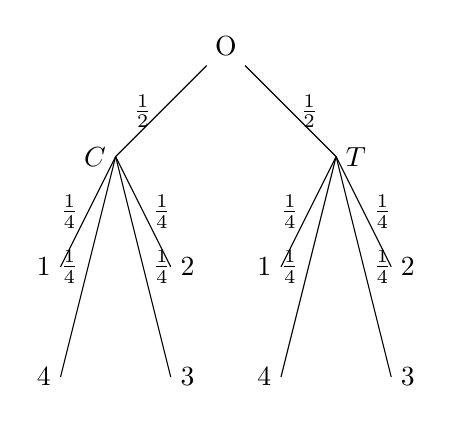
\begin{tikzpicture}[scale=0.7]
    \node (root) at (0,0) {O};
    \draw (root) -- (-2,-2) node[left] {$C$} node[midway,left] {$\frac{1}{2}$};
    \draw (root) -- (2,-2) node[right] {$T$} node[midway,right] {$\frac{1}{2}$};
    
    \draw (-2,-2) -- (-3,-4) node[left] {$1$} node[midway,left] {$\frac{1}{4}$};
    \draw (-2,-2) -- (-1,-4) node[right] {$2$} node[midway,right] {$\frac{1}{4}$};
    \draw (-2,-2) -- (-1,-6) node[right] {$3$} node[midway,right] {$\frac{1}{4}$};
    \draw (-2,-2) -- (-3,-6) node[left] {$4$} node[midway,left] {$\frac{1}{4}$};
    
    \draw (2,-2) -- (1,-4) node[left] {$1$} node[midway,left] {$\frac{1}{4}$};
    \draw (2,-2) -- (3,-4) node[right] {$2$} node[midway,right] {$\frac{1}{4}$};
    \draw (2,-2) -- (3,-6) node[right] {$3$} node[midway,right] {$\frac{1}{4}$};
    \draw (2,-2) -- (1,-6) node[left] {$4$} node[midway,left] {$\frac{1}{4}$};
\end{tikzpicture}

  \[
  \begin{aligned}
    & T = \text{"esito del lancio moneta e testa"} \\
    & C = \text{"esito del lancio moneta è croce"} \\
    & D_i = \text{"è uscito il numero } i \text{"} \\
    & P(C) = \frac{1}{2}, \quad P(T) = \frac{1}{2} \\
    & P(D_i | C) = \frac{1}{4} \\
    & P(D_i | T) = \frac{1}{4} \\
    & A = \text{"è uscito testa e il numero } i \text{"} \\
    & P(A) = P(T) \cdot P(D_i | T) = \frac{1}{2} \cdot \frac{1}{4} = \frac{1}{8} \\
    & \text{Analogamente per } C \cap D_i
  \end{aligned}
  \]
}

\subsection{Formula di Bayes}
Quando si deve calcolare una probabilità condizionata di eventi "nell'ordine temporale sbagliato", ad esempio se si calcolare $P(A|B)$ ma si conosce solo $P(B|A)$, si può utilizzare uno strumento utilissimo facilmente derivabile dalla matematica della probabilità condizionata, ovvero la formula di Bayes:

\thm{Formula di Bayes}{
  Siano $A$ e $B$ due eventi tali che $\mathbb{P}(A)>0$ e $\mathbb{P}(B)>0$, allora:
  \[
    \mathbb{P}(A|B) = \frac{\mathbb{P}(B|A)\mathbb{P}(A)}{\mathbb{P}(B)}
  \]
}
\pf{Dimostrazione}{

  Per definizione di $\mathbb{P}(A|B)$ si ha:
  \[
    \mathbb{P}(A|B) = \frac{\mathbb{P}(A \cap B)}{\mathbb{P}(B)}
  \]
  Utilizzando la regola della catena possiamo rimuovere il numeratore come segue:
  \[
    \mathbb{P}(A\cap B) = \mathbb{P}(B|A)\mathbb{P}(A)
  \]
  Quindi:
  \[
    \mathbb{P}(A|B) = \frac{\mathbb{P}(A \cap B)}{\mathbb{P}(B)} = \frac{\mathbb{P}(B|A)\mathbb{P}(A)}{\mathbb{P}(B)}
  \]
}


\ex{4.1}{
Ci sono due urne: la prima urna contiene una pallina bianca e due palline
rosse, mentre la seconda contiene due palline bianche e cinque palline rosse. Si lancia una
moneta: se esce testa si estrae una pallina dalla prima urna, se esce croce si estrae una
pallina dalla seconda.
Sapendo che `e stata estratta una pallina bianca, calcolare la probabilit`a che l’esito del
lancio della moneta sia stato testa.

EVENTI

$ T = \text{esce testa} $

$ B = \text{estrazione pallina bianca} $

$ \Omega = \{t,c\} \times \{b,r\} $

$ \mathbb{P}(T|B) = \frac{P(B|T)P(T)}{P(B)} = \frac{P(B|T)P(T)}{P(B|T)P(T)+P(B|T^{c})P(T^{c})} = \frac{1/3 \cdot 1/2}{1/3 \cdot 1/2 + 2/7 \cdot 1/2} $ probabilita' totali e bayes
}

\ex{}{
Esempio 5.1. In un’urna ci sono due palline che possono essere rosse (R) o bianche (B).
La composizione esatta non `e nota, quindi le composizioni possibili sono:
RR, RB, BB. (H0, H1, H2)
Supponiamo che, in base alle informazioni a disposizione, sia ragionevole assegnare uguale
probabilit`a pari a 1/3 alle tre composizioni (ipotesi) possibili, che denotiamo H0, H1 e H2.
1) Se si estrae una pallina dall’urna, qual `e la probabilit`a che sia bianca?
2) Si effettuano tre estrazioni con reimmissione: sapendo che le prime due palline
estratte sono bianche, qual `e la probabilit`a che anche la terza pallina estratta sia
bianca?

Il paradosso viene dal fatto che dobbiamo tenere traccia dell'asimmetria iniziale e denotare le diverse composizioni come ipotesi possibili.

EVENTI

$ B_i = \text{estraggo una pallina bianca all'i-esima estrazione} $

1) $ P(B_1) = P(B_1|H_0)P(H_0) + P(B_1|H_1)P(H_1) + P(B_1|H_2)P(H_2) = 1/2 $ probabilita' totali e prob. unifore delle H

Ce l'aspettiamo dato che c'e' completa simmetria fra i rami delle H con la distribuzione di palline

2) $ P(B_3 | B_1 \cap B_2) = P(B_3 \cap B_2 \cap B_1) / P(B_1 \cap B_2) =  $ usare ancora il partizionamento per H per applicare probabilita' totali
}

% \end{document}

% \begin{document}
\chapter{Calcolo Combinatorio}  

Quando abbiamo numero finito di elementi con probabilita' uniforme, e' possibile utilizzare l'addittivita' delle probabilita' per ridurre il problema di probabilita' a un problema di conteggio (la probabilita' di un evento e' data dal numero di casi favorevoli) $ \implies $ dobbiamo imparare a contare.

Dato un certo insieme, dobbiamo calcolarne la cardinalita' utilizzando i giusti stumenti matematici:

\thm{Calcolo probabilita' uniforme (Laplace)}{
  Se $ \Omega $ e' finito, $ \Omega = \{w_1,...,w_N\} $ e $ \forall i = 1,...,N.\ \mathbb{P}(\{w_i\}) = \frac{1}{N} $ (probabilita' uniforme), allora $ \forall A \subseteq \Omega $ (evento):
  \[
    \mathbb{P}(A) = \frac{|A|}{N}
  \]
}

Dobbiamo introdurre:
\begin{itemize}
\item \textbf{Fattoriali}:
  \begin{itemize}
  \item $ 0! \coloneq 1 $
  \item $ (n+1)! \coloneq (n+1) \cdot n! $
  \end{itemize}
  \item \textbf{Coefficenti Binomiali}:
    \[
      \binom{n}{k} = \frac{n!}{k! (n-k)!} \quad \forall n,k\in \mathbb{N}. n \geq k
    \]
    In generale:
    \[
      \binom{n}{k} = \binom{n}{n-k}
    \]
    Dal triangolo di Tartaglia, possiamo visualizzare altre proprieta' (oltre alla simmetria)
\end{itemize}

Vedremo che $ \binom{n}{k} $ sono il numero di modi diversi che abbiamo per selezionare $ k $ sottoinsiemi diversi da un insieme di cardinalita' $ n $.

\thm{Formula di Newton}{
  \[
    (a+b)^n = \sum_{k=0}^{n} \binom{n}{k} a^k b^{n-k}
  \]
}

Quindi anche il coefficente deriva da un problema di conteggio.

\section{Metodo (Principio) delle Scelte Successive}
E' un algoritmo per determinare la cardinalita' di un insieme. Vediamo un esempio:
\ex{}{
  Alfabeto di 36 caratteri dove ognuno dei numeri corrisponde a un carattere alfanumerico.

  \underline{Domanda}: "Quante possibili password distinte di 8 caratteri esistono in questo alfabeto?"

  $ \Omega = \text{Alfanumerici} \times ... \times \text{Alfanumerici} $ 8 volte.

  \begin{itemize}
  \item Scelte:
    \begin{enumerate}
    \item un carattere dei 36 totali
    \item \vdots (e' cosi 8 volte)
    \end{enumerate}
    Quindi $ |\Omega| = 36 \times ... \times 36 = 36^8 $
  \end{itemize}

  E se vogliamo evitare di ripetere i caratteri? Vediamo le scelte:
  \begin{enumerate}
  \item un carattere dei 36 totali
  \item un carattere dei \textbf{35 possibili}
  \item \vdots
  \item un carattere dei 29 possibili
  \end{enumerate}
  Quindi $ |\Omega| = 36 \times 35 \times \dots \times 29 = \frac{36!}{28!} $
}

Definiamo il principio generale:

\thm{Non proprio un teorema}{
  Ciascun elemetno di un insieme $ A $ puo' essere determinato tramite sola sequenza di $ k $ scelte, dove per ogni scelta ci sono $ n_1,\dots,n_k $ possibilità, allora:
  \[
  |A| = n_1 \times \dots \times n_k
  \]
}

\nt{
  Puo' essere riscritto come teorema formale ma \textbf{E' TROPPO DIFFICILE PER NOI INFORMATICI} quindi non lo facciamo!!!!
}

\ex{}{
  52 carte (13 tipi 4 semi)
  \begin{enumerate}
    \item $ A = \text{iniseme dei full (un tris e una coppia)} $, $ |A| = ? $

      \underline{4 scelte:}
      \begin{itemize}
        \item tipo di carta nel tris (13)
        \item tipo di carta nella coppia (12)
        \item semi nel tris (4)
        \item semi nella coppia (6)
      \end{itemize}
      $ |A| = 13 12 4 6 = \text{casi favorevoli} $

    \item $ A = \text{doppie coppie (due coppie di tipo diverso e una carta libera)} $, $ |A|=? $

      \underline{Scelte}:
      \begin{itemize}
        \item tipo nella prima coppia (13)
        \item tipo nella seconda coppia (12)
        \item semi nella prima coppia (6)
        \item semi seconda (6)
        \item tipo singolo (11)
        \item seme singolo (4)
      \end{itemize}
      $ |A| = 13 12 6 6 11 4 $ \textbf{SBAGLIATO!!}

      Perche' non ci interessa dell'ordine delle due coppie (bisogna dedurlo dalla definizione di A), quindi NON c'e' una prima e seconda coppia (anche sopra era sbagliato vederlo cosi') dato che non c'e' l'ordine.

      Combinazioni dei tipi che compongono 2 coppie ($ 13 \times 12 / 2 $)
  \end{enumerate}
}

\section{Disposizioni}

\dfn{Disposizioni con ripetizione}{
  Dato un insieme $ E $ con $ n $ elementi, indichiamo con $ DR_{n,k} $ le sequenze ordinate di $ k $ elementi di $ E $. }
Sostanzialmente, $ DR_{n,k} = E \times E ... \times E $ $ k $ volte, ovvero:
\[
DR_{n,k} = E^k
\]
Quindi usando il principio delle scelte successive:
\[
|DR_{n,k}| = n^k
\]
dato che per ogni $ E $ abbiamo una scelta fra $ n $ elementi.

\nt{
  Indicando tale insieme con $ DR_{n,k} $, l'insieme $ E $ sparisce, dato che ci interessa solo la \textbf{cardinalita'} di tale insieme e non ce ne frega un cavolo dei sui elementi.
}

\ex{Iniziamo a calcolare le probabilita'!}{
  Presa un urna con $ n $ palline numerate ($ E = \{1,...,n\} $) e si estraggono $ k $ palline con \textit{reinbussolamento}.
  \[
  \Omega = E \times ... \times E = DR_{n,k}
  \]
  Quindi $ |\Omega| = n^k $, e la probabilita' uniforme e' data da:
  \[
    \mathbb{P}(\{\omega\}) = \frac{1}{|\Omega|} = n^{-k}
  \]
}
\ex{}{
  Determinare spazi campionari per i seguenti esperimenti:
  \begin{itemize}
  \item Scelta casuale di una parola di 8 lettere
  \item Scelta di colonne deltotocalcio (risultato di 13 partite)
  \end{itemize}
}

Quindi lo usiamo nei casi di estrazione con reinbussolamento quando ci interessa l'ordine.

\dfn{Disposizioni}{
  Dato un insieme $ E  $ di $ n $ elementi, l'insieme delle disposizioni (senza ripetizione) di $ k $ elementi dell'insieme $ E $ e' l'insieme delle sequenze ordinate di $ k $ elementi \textit{distinti}, ovvero:
  \[
    D_{n,k} \coloneq \{(x_1,...,x_k)|x_1,...,x_k \in E \land x_i \neq x_j \text{se} i \neq j \}
  \]
}

\nt{
  $ D_{n,k} $ e' un sottoinsieme \textbf{stretto} di $ DR_{n,k} $.
}

Usando le scelte successive:
\[
  |D_{n,k}| = n\times (n-1) \times ... \times (n-k+1) = \frac{n!}{(n-k)!}
\]
L'esperimento aleatorio di riferimento e' l'estrazione \textbf{senze} reimissione.

\dfn{Permutazioni}{
  $ P_n = D_{n,n} $, quindi:
  $ |P_n| = n! $
}

\section{Combinazioni}
\dfn{Combinazioni}{
  Dato un insieme $ E $ di $ n $ elementi, indichiamo con $ C_{n,k} $ la classe dei sottoinsiemi di $ E $ contenenti $ k $ elementi, ovvero:
  \[
  C_{n,k} = \{A \subseteq E \mid |A|= k\}
  \]
}
Siamo passati da sequenze a sottoinsiemi, ovvero non ci interessa piu' dell'ordine:
\[
\text{sottoinsieme} = \text{sequenza non ordinata}
\]



\mprop{sulla combinazione come coefficiente biniomiale}{
  Sia la combinazione $C_{n,k}$, allora vale:
  \begin{equation}
    |C_{n,k}| = \binom{n}{k}
  \end{equation}
}
\pf{Dimostrazione}{
  Mi riduco a dimostrare che:
  \[
    \frac{n!}{(n-k)!} = |C_{n,k}|k!
  \]
  Ovvero
  \[
    |D_{n,k}| = |C_{n,k}|\cdot |P_k|
  \]



  Ma $|D_{|n,k|} = |C_{n,k}|\cdot |P_k|$ vale per il principio delle scelte successive, infatti:
  \begin{itemize}
    \item scelta per i $k$ elementi selezionati: $|C_{n,k}|$
    \item scelta dell'ordinamento $|P_k|$
  \end{itemize}
}

Si noti questo esempio

\ex{}{
  Consideriamo un'unrna con $n$ palline distinte delle quali ne vengono estratte $k$. Determinare lo spazio di probabilità
  
  \hrule
  
  Si ha che: $\Omega = C_{n,k}$

  Mentre per il principio di probabilià uniforme si ha:
  \[
    \mathbb{P}(\{w\}) = \frac{1}{\binom{n}{k}} = \frac{k!(n-k)!}{n!}
  \]
}

Interpretazione combinatoria della formula di Stifel
\nt{
  Si consideri la formula di Stifel:
  \begin{equation}
    \binom{n}{k} = \binom{n-1}{k-1} + \binom{n-1}{k}
  \end{equation}
  Si può interpretare questa formula in termini di combinazioni come segue:

  \[
    \underbrace{\binom{n}{k}}_{\parbox{4cm}{n° di combinazioni di $k$ elementi di $E$}} = 
    \underbrace{\binom{n-1}{k-1}}_{\parbox{4cm}{n° di combinazioni di $k$ elementi di $E$ in cui è presente l'elemento $\bar{e}$}} + 
    \underbrace{\binom{n-1}{k}}_{\parbox{4cm}{n° di combinazioni di $k$ elementi di $E$ senza l'elemento $\bar{e}$}}
  \]
  dove $\bar{e}$ è un elemento fissato
}

Interpretazione combinatoria del binomio di Newton
\nt{
  Si consideri la formula del binomio di Newton:
  \begin{equation}
    (a+b)^n=\sum_{k=0}^n\binom{n}{k}a^kb^{n-1}\quad a,b\in \mathbb{R}
  \end{equation}

  Il prodotto $(a + b)(a + b)\dots(a + b)$ di $n$ fattori si sviluppa in una somma di monomi di grado $n$ del tipo $a^{n-k}b^k$ dive $k$ varia da 0 a $n$. Dobbiamo quindi determinare il coefficente di ogni monomio  $a^{n-k}b^k$, ossia calcolare quante volte compare facendo il prodotto $(a+b)(a+b)\dots (a+b)$ ossia calcolare quante volte compare facendo il prodotto $(a+b)(a+b)\dots (a+b)$. Questo monomio però si ottiene sciegliendo il valore $b$ da $k$ degli $n$ fattori e $a$ dai rimanenti $n-k$, ovvero in $\binom{n}{k}$ modi
}

\section{Tipologie di esperimenti}
Riassumendo, si possono verificare 3 casi notevoli durante un esperimento aleatorio inseriti in questa tabella
  
\begin{table}[h]
  \centering
    \begin{tabular}{|m{5cm}|m{5cm}|m{5cm}|}
    \hline
    % \backslashbox{\textbf{ORDINE}}{\textbf{RIPETIZIONE}} & \textbf{Senza ripetizione} & \textbf{Con ripetizione} \\ TODO: porcodio perche' e' tornato cosi'? L'avevo messo a posto 
    \hline
    Si tiene conto dell'ordine & 
    \begin{tabular}{@{}l@{}}
    Estrazione senza reimmissione \\
    $\Omega = \mathsf{D}_{n,k}$ \\
    $|\Omega| = \dfrac{n!}{(n-k)!}$
    \end{tabular} &
    \begin{tabular}{@{}l@{}}
    Estrazione con reimmissione \\
    $\Omega = \mathsf{DR}_{n,k}$ \\
    $|\Omega| = n^k$
    \end{tabular} \\ 
    \hline
    Non si tiene conto dell'ordine & 
    \begin{tabular}{@{}l@{}}
    Estrazione simultanea \\
    $\Omega = \mathsf{C}_{n,k}$ \\
    $|\Omega| = \dfrac{|\mathsf{D}_{n,k}|}{k!} = \binom{n}{k}$
    \end{tabular} & --- \\ 
    \hline
    \end{tabular}
    \caption{Gli spazi campionari e le loro cardinalità.}
  \label{tab:spazi_campionari}
\end{table}


\nt{
  La casella vuota nella tabella sopra riportata corrisponde all’insieme delle cosiddette \textit{combinazioni con ripetizione}, un raggruppamento di $k$ elementi estratti da $n$ elementi distinti, nel quale uno stesso elemento può ripetersi fino a $k$ volte, e in cui l'ordine di estrazione non è rilevante
}

Si noti questo esempio:
\ex{Esempio sulla casella mancante}{
  si lancia tre volte una moneta. Qual è la probabilità che esca due volte testa?

  \hrule

  Si hanno due approcci per scegliere lo spazio campionario:
  \begin{itemize}
    \item utilizzare le $DR_{2,3}$ con $\mathbb{P}$ uniforme.
    
    In questo caso:
  
  \[
    \Omega =DR_{2,k} = \{(T, T, T), (T, T, C), (T, C, T), (C, T, T), (T, C, C), (C, T, C), (C, C, T), (C, C, C)\}
  \]

  Ci sono 8 possibili sequenze perché ogni lancio ha 2 possibili risultati:
  \[
    2^3 = 8
  \]
  Siccome ogni sequenza ha la stessa probabilità di verificarsi, possiamo assegnare la probabilità uniforme, si ha

  \[
    \mathbb{P}(x_1,x_2,x_3) = \frac{1}{8} \quad \forall x 
  \]

  Sarà quindi facile calcolare la probabilità di $A$ (lascio al basta come esercizio)
  \item Lo spazio campionario con combinazioni con ripetizione $CR_{n,k}$.
  
  In questo caso, dato che non ci interessa l'ordine dei lanci, dobbiamo raggruppare le sequenze "uguali":

  \[
    CR_{2,3} = \{[T,T,T],[T,T,C],[T,C,C],[C,C,C]\}
  \]

  Tuttavia è facile verificare che in questo caso la probabilità uniforma \textbf{non sussiste}, perché alcuni gruppi contengono più sequenze di altri

  infatti:

  \begin{itemize}
    \item $\mathbb{P}([T, T, T]) = \P((T, T, T)) =\frac{1}{8}$
    \item  $\P([T, T, C]) = \P((T, T, C)) + \P((T, C, T)) + \P((C, T, T))=\frac{3}{8}$
    \item $\P([T, C, C]) = \P((T, C, C)) + \P((C, T, C)) + \P((C, C, T)) =\frac{3}{8}$
    \item $\mathbb{P}([C,C,C]) = \P((C,C,C)) =\frac{1}{8}$
  \end{itemize}
\end{itemize}
}

\nt{
  Se scegliamo lo spazio campionario $CR_{n,k}$, dobbiamo lavorare con probabilità non uniformi, il che complica i calcoli.Invece, se lavoriamo con , tutte le sequenze hanno la stessa probabilità e possiamo usare il calcolo combinatorio standard per trovare i risultati.

  Per questo motivo, nella maggior parte dei problemi in cui c’è ripetizione, conviene lavorare con disposizioni con ripetizione , perché permette di usare la probabilità uniforme.
}

Bho adesso si fa un altro esempio, e va benissimo così

\ex{Probabilità binomiale}{
  Si consideri un’urna che contiene $b$ palline bianche ed $r$ palline rosse. Si effettuano $k$ estrazioni con reimmissione. Calcolare la probabilità dell’evento

  \[
    A_\ell = \text{"si estraggono } \ell \text{ palline bianche ed } k - \ell \text{ palline rosse''}
  \]
}

\pf{soluzione}{
  Etichettiamo le $b$ palline bianche con $b_1,b_2, \dots, b_b$; analogamente, le $r$ palline rosse con $r_1,\dots , r_r$. Sia dunque:
  \[
    E = \{b_1,\dots, b_b,r_1,\dots , r_r\}
  \]

  E si noti che $|E| = b+r$.

  Come spazio di probabilità $(\Omega,\P)$ è naturale considerare $\Omega = DR_{b+r, k}$ (insieme delle disposizioni con ripetizione di $k$ elementi di $E$) e $\P$ probabilità uniforme, quindi $\P(\{w\})=\frac{1}{(b+r)^n}$

  Per calcolare $\P(A_\ell)$ dobbiamo calcolare $|A_\ell|$ che si rivela possibile usando il principio delle scelte successive:
  \begin{itemize}
    \item scelta della sequenza di $\ell$ palline bianche estratte, ovvero $|DR_{b,\ell}|$ possibilità
    \item scelta della sequenza di $k-\ell$ palline bianche estratte, ovvero $|DR_{b,k-\ell }|$ possibilità
    \item scelta delle $\ell$ estrazioni in cui sono uscite le palline bianche: $|C_{k,\ell}|$ possibilità
  \end{itemize}

  In defintiva:
  \[
    \P(A_\ell) = \frac{|DR_{b,\ell}||DR_{b,k-\ell }||C_{k,\ell}|}{| DR_{b+r, k}|} = \binom{k}{\ell}\frac{b^\ell r^{k-\ell}}{(b+r)^k}
  \]
  O, equivalentemente, dato $p=\frac{b}{b+r}$ si ha:
  \[
    \P(A_\ell) = \binom{k}{\ell}p^\ell (1-p)^{k-\ell}, \quad \ell = 0,\dots, k
  \]
}

\nt{
  Consideriamo lo spazio di probabilità $(\Omega, \mathbb{P})$ con $\Omega = \{0, 1, 2, ..., k\}$ e $\mathbb{P}$ data da
\[
\mathbb{P}(\{\ell\}) = \binom{k}{\ell} p^\ell (1-p)^{k-\ell}, \qquad \ell = 0, 1, ..., k.
\]

Si noti che $\mathbb{P}$ è effettivamente una probabilità. Infatti, per la formula del binomio di Newton vale che
\[
\sum_{\ell=0}^k \mathbb{P}(\{\ell\}) = \sum_{\ell=0}^k \binom{k}{\ell} p^\ell (1-p)^{k-\ell} = (p + (1-p))^k = 1.
\]

$\mathbb{P}$ non è una probabilità uniforme. $\mathbb{P}$ si chiama \textbf{probabilità binomiale}.





}

% \begin{document}
\chapter{Variabili Aleatorie}
\section{Introduzione}
  Finora, abbiamo trattato solo di eventi, per i quali ci chiediamo, fatto l'esperimento aleatorio, se sono avvenuti o meno. Possiamo pensare di domandarci non se un'affermazione si realizza o meno, ma generalizzare l'idea e chiederci quale sara' la quantita' numerica aleatoria, associata quindi ad un esperimento. Vogliamo quindi formalizzare l'idea di una quantita' che dipende dall'esito di un esperimento aleatorio:
  \dfn{Variabile Aleatoria}{
    Diamo due affermazioni (come per gli eventi):
    \begin{itemize}
    \item \textbf{Affermazione}:

      Una variabile aleatoria e' un'affermazione che riguarda il risultato dell'esperimento aleatorio. Tale affermazione identifica uno e un solo numero, una volta noto l'esito. Stiamo quindi rispondendo alla domanda "Quanto vale ... ?"

      \item \textbf{Funzione}:

        Dato uno spazio di probabilita' $ (\Omega, \mathbb{P}) $ ed un insieme $ E \neq \emptyset $, si dice \textit{variabile aleatoria} ogni funzione $ X $ del tipo:
        \[
        X: \Omega \to E
        \]
        Se $ E = \mathbb{R} $, allora $ X $ e' una variabile aleatoria \textit{reale}. Puo' anche essere che $ E = \mathbb{R}^{n} $ con $ n > 1 $, e in questo caso si parla di variabili aleatorie \textit{vettoriali}.
      
    \end{itemize}
  }

  \ex{Lancio di due dadi}{
    Dato lo spazio di probabilita', definiamo una variabile aleatoria $ X $:
    \[
    X = \text{La somma dei due lanci}
    \]
    Dobbiamo, quindi, prendere l'esito dell'esperimento e sommare il valore dei due dadi. Questa operazione puo' essere vista come una funzione a cui viene passata l'esito dell'esperimento e che restituisce un numero reale:
    \begin{align*}
      X: \Omega \to \mathbb{R}
    \end{align*}
    Questa e' la definizione di variabile aleatoria come funzione.

    In questo caso, $ \Omega = \{1,...,6\}\times \{1,...,6\} = DR_{6,2} $, qundi:
    \[
      X((\omega_1, \omega_2)): \omega_1+\omega_2
    \]
  }
  \nt{
    Qualunque funzione da $ \Omega $ a $ \mathbb{R} $ e' una variabile aleatoria. Se $ \Omega $ e' piu' che numerabile sorgono dei problemi a causa dell'unione numerabile, quindi viene usata la $ \sigma $-algebra, un insieme delle parti ristretto per evitare tali problemi. 
  }

  \section{Variabili Aleatorie Costanti}
  Vediamo dei casi "banali" di variabili aleatorie per capire il loro funzionamento e come vengono definite. Iniziamo con le funzioni costanti:
  \dfn{Variabile Aleatoria Costante}{
    Una VA (variabile aleatoria) $ X $ si dice \textit{costante} se:
    \[
      \forall \omega \in \Omega.\ X(\omega) = a
    \]
    Dove $ a \in E $ e' un elemento fissato. E' definita $ \forall \Omega $, dato che e' deterministica (non dipende dall'esito dell'esperimento).
  }
  Come per gli eventi, anche le variabili aleatorie possono essere \textit{quasi} costanti:
  \dfn{Variabili Aleatorie Quasi Costanti}{
    Una VA $ X $ si dice \textit{quasi costante} se:
    \[
      \forall \omega \in \Omega.\ \mathbb{P}(X = a) = 1
    \]
  }
  \nt{
    La scrittura $ (X = a) $ e' una notazione che rappresenta l'evento $ A = \text{"Il valore di X sara' "} a $, ovvero il sottoinsieme di $ \Omega $ per cui tutti gli elementi, passati a $ X $, danno lo stesso valore $ a $, quindi:
    \[
      \mathbb{P}(X = a) \coloneq \mathbb{P}(\{\omega \in \Omega | X(\omega) = a\})
    \]
  }
  \ex{Lancio di un dado}{
    $ \Omega = \mathbb{R} $, $ \mathbb{P} $ probabilita' uniforme su $ \{1,...,6\} $ e nulla sul resto degli elementi.

    Con $ E = \mathbb{R} $, fisso $ a \in E $ e voglio costruire $ X: \Omega \to E $ tale che $ X $ e' quasi costante:
    \[
      X(\omega) = \begin{cases}
      a & \omega \in \{1,...,6\}\\
      \omega & \text{altrimenti}
      \end{cases}
    \]
    Questa e' effettivamente una VA quasi costante, dato che $ \mathbb{P}(X = a) = 1 $. Infatti abbiamo assegnato un valore costante $ a $ a tutti gli $ \omega $ la cui probabilita' non era nulla. Ricordiamoci che la notazione $ \mathbb{P}(X = a) $ puo' essere riscritta meglio come $ \mathbb{P}(\{\omega \in \Omega | X(\omega) = a\}) $, che in questo caso corrisponde con $ \mathbb{P}(\{1,...,6\}) $ che ovviamente e' uguale a 1.

    Notare che per tutti gli $ \omega $ con probabilita' nulla, il valore di $ X $ associato puo' essere qualunque cosa (non costante) e la $ X $ rimane comunque quasi costante. 
  }

  \section{Variabili Aleatorie Indicatrici (o di Bernulli)}

  \dfn{Varaibile Aleatoria Indicatirce}{
    Dato un evento $ A \subseteq \Omega $, definisco la variabile aleatoria indicatrice di $ A $ come:
    \[
      X(\omega): \mathbb{1}_A(\omega) = \begin{cases}
      1 & \omega \in A\\
      0 & \omega \notin A
      \end{cases}
    \]
  }
  Quindi, dato un evento, la VA indicatrice $ X $ ci \textit{indica} se l'esito $ \omega $ appartenga o meno all'evento. Notiamo che tutta l'informazione dell'evento $ A $ e' contenuta nella VA:
  \[
  A \rightsquigarrow \mathbb{1}_A
  \]
  Allora le VA sono \textit{generalizzazioni} del concetto di evento.

\ex{Prove ripetute e indipendenti}{
  Consideriamo uno schema di $n$ prove ripetute e indipendenti con probabilità di successo $p$, ossia uno spazio di probabilità discreto $(\Omega, P)$ in cui sono definiti $n$ eventi $C_1, \ldots, C_n$ indipendenti e con la stessa probabilità $p = P(C_i)$ (si ricordi il Paragrafo 1.3.4). Nel Paragrafo 1.3.4.3 abbiamo studiato gli eventi

  \begin{align*}
    A_k &:= \text{``esattamente $k$ prove hanno successo''}, \\
    B_\ell &:= \text{``il primo successo si verifica nella $\ell$-esima prova''},
  \end{align*}
    
  per $0 \leq k \leq n$ e $1 \leq \ell \leq n$. Introduciamo ora due variabili aleatorie
    
  \begin{align*}
    S &:= \text{``numero di successi nelle $n$ prove''}, \\
    T &:= \text{``prova in cui si ha il primo successo''},
  \end{align*}
    
  definite su $\Omega$ a valori rispettivamente in $\{0, 1, \ldots, n\}$ e in $\mathbb{N} \cup \{+\infty\}$, mediante
    
  \begin{equation}
    S(\omega) := \sum_{i=1}^{n} 1_{C_i}(\omega), \quad T(\omega) := \min\{i \in \{1, \ldots, n\} : \omega \in C_i\},
  \end{equation}
    
  con la convenzione $\min \emptyset := +\infty$. Possiamo allora esprimere gli eventi $A_k$ e $B_\ell$ nel modo seguente:
    
  \begin{equation}
    A_k = \{\omega \in \Omega : S(\omega) = k\}, \quad B_\ell = \{\omega \in \Omega : T(\omega) = \ell\}.
  \end{equation}
    
  Questo mostra che gli eventi $A_k$ e $B_\ell$ possono essere definiti in modo naturale in termini delle variabili aleatorie $S$ e $T$, specificandone un sottoinsieme di valori.
    
}

  \section{Eventi associati alle variabili aleatorie}

  Ma se io ho $ X $ variabile aleatoria, sono capace di risalire all'evento (o eventi) associati? Le variabili aleatorie sono generalizzazioni del concetto di evento, quindi data una variabile aleatoria ci sono una moltitudine di eventi associati (o generati)

  \dfn{Evento generato da una VA}{
    Sia $ X: \Omega \to E $ una VA. $\forall A \subseteq \mathbb{R} $ indichiamo con $ \{X \in A\} $ la controimmagine di $ A $ tramite $ X $:
    \[
      \{X \in A\} \coloneq X^{-1}(A) = \{\omega \in \Omega | X(\omega) \in A\}
    \]
    Quindi $ \{X \in A\} \subseteq \Omega $ e' un evento, ed e' costituito da tutti e soli gli esiti $ \omega $ per cui $ X(\omega) \in A $.

    Gli eventi di questo tipo si dicono \textit{generati da} $ X $.
  }

  \nt{
    La scrittura $ \{X = a\} $ che abbiamo usato prima e' equivalente a scrivere $ \{X \in \{a\}\} $. Allo stesso modo, possiamo considerare un intervallo di valori usando le disequazioni: $ \{X > a\} \equiv \{X \in (a,+\infty)\} $.
  }

  Segue quindi:
  \dfn{Insieme di eventi generati da una VA}{
    Data una VA $ X $, l'insieme degli eventi da essa generati si indica con:
    \[
      \sigma(X) \coloneq \{\{X \in A\} | A \subseteq \mathbb{R}\} \subseteq \powerset(\Omega)
    \]
  }

  \nt{
    $ \forall X: \Omega \to \mathbb{R} $ v.a. possiamo scrivere:
    \[
    \Omega = \{X \in \mathbb{R}\}
    \]
    \[
    \emptyset = \{X \in \emptyset\}
    \]
  }

  Calcoliamo l'insieme degli eventi generati dalle VA particolari che abbiamo visto:

  \begin{itemize}
  \item $ X $ \textbf{costante}:

    Fisso $ a \in \mathbb{R} $, tale che $ \forall \omega \in \Omega.\ X(\omega) = a $.

    $ \sigma(X) = ? $

    Fissato $ B \subseteq \mathbb{R} $, notiamo che ci sono solo due casi:
    \[
    \{X \in B\} = \begin{cases}
    \Omega & a \in B\\
    \emptyset & a \notin B
    \end{cases}
    \]
      Infatti, se $ a $ appartiene a $ B $ allora $ \forall \omega \in \Omega.\ X(\omega) \in B $ e quindi $ \{X \in B\} = \Omega $. Mentre se $ a $ non appartiene a $ B $, si ha che $ \forall \omega \in \Omega.\ X(\omega) \notin B $ e quindi $ \{X \in B\} = \emptyset $.
  \item $ X $ \textbf{indicativa}:

    Fisso $ A \subseteq \Omega $ tale che $ \forall \omega \in \Omega.\ X(\omega) = \mathbb{1}_A(\omega) $.

    $ \sigma(X) = ? $

    Fissato $ B \subseteq \mathbb{R} $, vediamo i casi:
      \[
      \{X \in B\} = \begin{cases}
      \Omega & 0 \in B \land 1 \in B\\
      \emptyset & 0 \notin B \land 1 \notin B\\
      A & 0 \notin B \land 1 \in B\\
      A^{c} & 0 \in B \land 1 \notin B
      \end{cases}
      \]
  \end{itemize}   

  \mprop{}{
    Sia $ X: \Omega \to \mathbb{R} $ VA su $ (\Omega, \mathbb{P}) $, allora $ \forall x \in \mathbb{R} $:
    \begin{enumerate}
      \item $ \mathbb{P}(\{X \geq a\}) = \mathbb{P}(\{X = a\}) + \mathbb{P}(\{X > a\}) $
      \item $ \mathbb{P}(\{X \geq a\}) = 1 - \mathbb{P}(\{X < a\}) $
    \end{enumerate}
  }
  \pf{}{
    \begin{enumerate}
      \item $ \{X \geq a\} = \{ \omega \in \Omega | X(\omega) > a \lor X(\omega) = a\} = \{X > a\} \uplus \{X = a\} $ dato che se $ X(\omega) > a $ allora $ X(\omega) \neq a $ e viceversa. Quindi l'equazione e' dimostrata per addittivita' finita.
      \item Dimostriamo che $ \{X \geq a\} $ e $ \{X < a\} $ sono complementari. Se $ X(\omega) \not\geq a $, allora $ X(\omega) < a $ e viceversa, fatto.
    \end{enumerate}
  }

   Possiamo confronare intervalli su $ \mathbb{R} $ per calcolare probailita'

 \section{Distribuzione (o legge) di una Variabile Aleatoria}

 Ora che sappiamo trovare l'evento generato da una variabile aleatoria e un sottoinsieme del suo codominio, possiamo calcolare la probabilita' di tale evento: 

 \dfn{Distribuzione di una VA}{
   Dati $ (\Omega, \mathbb{P}) $ e $ X: \Omega\to \mathbb{R} $ VA, chiamiamo legge di $ X $ la funzione:
   \begin{align*}
     \mathbb{P}_X: \powerset(\mathbb{R}) &\to [0,1]\\
     B &\mapsto \mathbb{P}(X \in B)
   \end{align*}
   Si scrive $ X \sim \mathbb{P}_X $ e si legge "$ X $ ha legge $ \mathbb{P}_X $".
 }
 \mprop{}{
   La distribuzione $ \mathbb{P}_X $ di una variabile aleatoria $ X: \Omega \to E $ e' una probabilita' sull'insieme $ E $. (per noi $ E $ sara' quasi sempre $ \mathbb{R} $).
 }
 La legge di una VA ne calcola quindi, dato un insieme di valori reali, la probabilita' che $ X(\omega) $ appartenga a tale intervallo. Quindi, anche senza conoscere la funzione $ X $, se conosciamo la sua distribuzione sappiamo quali valori puo' assumere e con quale probabilita'.

 Andiamo a costruire le distribuzioni delle VA "banali" studiate precedentemente:
  \begin{itemize}
  \item Variabili Costanti:

    $ a \in \mathbb{R}, X(\omega) = a.\ \forall \omega \in \Omega $

    \[
    B \subseteq \mathbb{R}.\ \{X \in B\} = \begin{cases}
    \Omega & a \in B\\
    \emptyset &  a \notin B
    \end{cases}
    \]
    \[
    \mathbb{P}_X(B) = \mathbb{P}(X \in B) = \begin{cases}
    1 & a \in B\\
    0 & a \notin B
    \end{cases}
    \]
      Questa e' la delta di Dirac di $ a $ valutata su $ B $
    \item Variabili Indicatrici:

      $ A \subseteq \Omega $, $ X(\omega) = \mathbb{1}_A(\omega) $
      \[
      B \subseteq \mathbb{R}, \{X \in B\} = \begin{cases}
      \Omega & 1, 0 \in B\\
      \emptyset & 1, 0 \notin B\\
      A & 1 \in B \land 0 \notin B\\
      A^{c} & 1 \notin B \land 0 \in B
      \end{cases}
      \]
      \[
        P_X(B) = P(X \in B) = \begin{cases}
        1 & 1,0 \in B\\
        0 & 1,0 \notin B\\
          P(A) & 1 \in B \land 0 \notin B\\
          1-P(A) & 1 \notin B \land 0 \in B
        \end{cases}
      \]
      Questa e' una probabilita' discreta, quidni e' possibile crearla usando una combinazione lineare di delta di Dirac: 
      \[
        = P(A)\delta_1(B) + (1-P(A))\delta_0(B)
      \]
      Ovvero:
      \[
        P_X(\cdot) = P(A)\delta_1(\cdot) + (1-P(A))\delta_0(\cdot)
      \]
      Distribuzione (o legge) di Bernulli. Se la variabile aleatoria diventa piu' complicata, aumentano il numero di delta.
\dfn{Distribuzioni di Bernulle}{
  $\P_x (\cdot) = \P(A) \delta_1(\cdot) + (1-\P(A))\delta_0(\cdot)$
}
  \end{itemize}

  \section{Funzione di Ripartizione}
  Molto bella la distribuzione di una VA, ma prende come input insiemi (sottoinsiemi di $ \mathbb{R} $) e questo ci complica un po' la vita. Vediamo una caratterizzazione piu' semplice che ci aiutera soprattutto per le VA assolutamente continue:
  \dfn{Funzione di Ripartizione}{
    Dati $ (\Omega, P) $ SP e una VA $ X: \Omega \to \mathbb{R} $, si chiama \textit{funzione di ripartizione} o \textit{CDF} di $ X $ la funzione:
    \begin{align*}
      F_X: \mathbb{R} &\to [0,1]\\
      x &\mapsto P_X((-\infty, x]) = P(X \leq x)
    \end{align*}
  }
 Diamo un'occhiata a come sono definite le funzioni di ripartizione per i soliti due casi "banali" di VA:
 \begin{itemize}
 \item VA Costanti:

   $ X(\omega) = a \implies P_X(B) = \delta_a(B) $, quindi la relativa funzione di ripartizione sara': 
  \[
  F_X(n) = P_X((-\infty, n]) = \delta_a(\{-\infty, n]) = \begin{cases}
  1 & n \geq a\\
  0 & n < a
  \end{cases}
  \]
    \begin{center}
      \includegraphics[width=0.5\textwidth]{img/2025-03-31-17-00-15.png}
    \end{center}
\item VA Indicatrici:

  $ X(\omega) = \mathbb{1}_A \implies P_X(B) = P(A)\delta_1(B) + (1-P(A))\delta_0(B) $, quindi la relativa funzione di ripartizione sara':
    \[
      F_X(x) = P_X((-\infty, x]) = P(A)\delta_1((-\infty, x]) + (1-P(A))\delta_0((-\infty, x])
    \]
     \[
     = \begin{cases}
     1 & x \geq 1\\
       1-P(A) & 0 \leq x < 1\\
     0 & x < 0
     \end{cases}
     \]
     \begin{center}
       \includegraphics[width=0.5\textwidth]{img/2025-03-31-17-13-24.png}
     \end{center}
 \end{itemize}

Teorema datoci dalla Shlein, che ci caratterizza la funzione di ripartizione:
\thm{Teorema di Teodoro}{
  $ (\Omega, P) $ SP, $ X: \Omega \to \mathbb{R} $, $ F_X $ fdr, allora:
  \begin{enumerate}
  \item $ F_X $ e' monotona crescente
  \item $ F_X $ e' continua a destra, ovvero $ \forall n \in \mathbb{R}.\ \lim_{y\to x^{+}} F_X(y) = F_X(n) $
  \item  $ \lim_{n \to +\infty} F_X(n) = 1 $
  \item $ \lim_{n\to -\infty} F_X(n) = 0 $
  \end{enumerate}

  Vale anche il viceversa: se $ G: \mathbb{R} \to [0,1] $ verifica 1,2,3,4, allora
  \[
    \exists(\Omega, P), X:\Omega\to \mathbb{R}.\ G \equiv F_X
  \]
}
\pf{}{
  \begin{itemize}
    \item 1) Devo dimostrare che $ \forall x,y \in \mathbb{R}, x < y.\ F_X(x) \leq F_X(y) $, ovvero che $ P_X((-\infty, x]) \leq P_X((-\infty, y]) $. Dato che $ (-\infty, n] \subset (-\infty, y] $ e col fatto che $ P_X $ e' una probabilia', e' dimostrabile usando la proprieta' di monotonia delle probabilita'.
    \item 2) 3) 4) Per queste dimostrazioni serve dimostrare prima la \textit{Stabilita' della Probabilita' per limiti monotoni}:
  \end{itemize}
}
\mlenma{}{
  Sia $ (\Omega, P) $ SP
  \begin{itemize}
    \item Data $ "A_x \uparrow A" $, ovvero una successione di eventi tali che $ A_x \subset A_{x+1}, \bigcup_{x=1}^{+\infty} A_x = A $, allora:
      \[
        \lim_{x\to+\infty} P(A_x) = P(A)
      \]
    \item Data $ "A_x \downarrow A" $, ovvero una successione di eventi tali che $ A_x \supset A_{x+1}, \bigcap_{x=1}^{+\infty} A_x = A $, allora:
      \[
        \lim_{x\to+\infty} P(A_x) = P(A)
      \]
  \end{itemize}

  Stessa roba per monotona al contrario
}
  Dato questo lemma, che non dimostriamo perche' si, possiamo concludere la dimostrazione precedente:
  \pf{}{
    3) Dobbiamo dimostrare che $ \lim_{x\to+\infty} P_X((-\infty, x]) = 1 $. Usiamo il lemma appena introdotto, dato che se poniamo $ A_x = (-\infty, x) $, possiamo creare una successione tale che $ A_x \uparrow \mathbb{R} $, per cui $ \lim_{x\to+\infty} P_X(A_x) = P_X(\mathbb{R}) = 1 $.

    Gli altri punti sono lasciati al DarioDestroyer04 come compito per casa
  }

    $ F_X $ e' continua a destra, quindi $ \lim_{y \to x^{+}}F_X(y) = F_X(x) = P(X \leq x)$. Inoltre si puo' dimostrare (usando il lemma) che esiste anche il limite sinistro e vale:
    \[
      \lim_{y\to x^{-}} F_X(y) = P(X < x)\ (F_X(x^{-}))
    \]
    Inoltre, sappiamo che:
    \[
      \underbrace{P(X \leq x)}_{F_X(x)} = \underbrace{P(X < x)}_{F_X(x^{-})} + \underbrace{P(X = x)}_{\Delta F_X(x)}
    \]
    \begin{center}
      \includegraphics[width=0.5\textwidth]{img/2025-03-31-19-35-15.png}
    \end{center}

    Quindi possiamo calcolare la probabilita' di ogni intervallo in termini della $ F_X $:
    \begin{itemize}
      \item $ (a,b] $: $ P_X((a,b]) = F_X(b) - F_X(a) $
      \item $ [a,b) $: $ P_X([a,b)) = F_X(b^{-}) - F_X(a^{-}) $
      \item $ (a,b) $: $ P_X((a,b)) = F_X(b^{-}) - F_X(a) $
      \item $ [a,b] $: $ P_X([a,b]) = F_X(b) - F_X(a^{-}) $
    \end{itemize}

 \nt{
   Conoscere $ \mathbb{P}_X $ $ \forall B \subseteq \mathbb{R} \iff$  conoscere $ \mathbb{P}_X $ $ \forall I $ intervallo di $ \mathbb{R} $, dato che:
   \begin{itemize}
   \item Ogni intervallo e' anche un'insieme
    \item Dato un sottoinsieme di $ \mathbb{R} $, questo puo' sempre essere scritto come unione di intervalli
   \end{itemize}

   Quindi, $F_X$ \textbf{determina completamente la distribuzione} di $X$, dato che ci da la distribuzione per tutti gli intervalli, e quindi per tutti gli insiemi.
 }

 \section{Variabili Aleatorie Discrete}

 Dato che ci stiamo concentrando sulle probabilita' discrete, ci conviene applicare la definizione \ref{dfn:probDiscr} anche per le VA:
 \dfn{Variabile Aleatoria Discreta}{
   Una VA $ X: \Omega \to E $ definita su uno spazio di probabilita' $ (\Omega, P) $ e' detta \textit{discreta} se esiste un sottoinsieme $ S_X \subset Im(X) $ finito o numerabile tale che:
   \[
     P_X(S_X) \coloneq P(X \in S_X) = 1
   \]
   Quindi un VA e' discreta sse la sua distribuzione e' una probabilita' discreta.

   Il sottoinsieme $ S_X $ e' chiamato supporto di $ X $.
 }

 \nt{
   Se $ \Omega $ o $ E $ sono finiti o numerabili, allora una VA definita su di essi sara' sicuramente discreto.
 }

 \subsection{Caratterizzazione delle VA discrete}
 Che relazione esiste tra $ p_X $ e la distribuzione di $ X $ ($ P_X $)? E tra $ p_X $ e $ F_X $?
 \subsubsection{Distribuzione}
 Essendo $ P_X $ una probabilita' discreta, possiamo definirla usando la Delta di Dirac:

 Sia $ S_X = \{x_1,...,x_n\} $ il supporto di $ X $, allora $ \exists p_1,...,p_n \in (0,1], \sum_{i=1}^{n} p_i = 1 $ tale che:
 \[
   \forall B \subseteq E.\ P_X(B) = \sum_{i=1}^{n} p_i \delta_{x_i}(B)
 \]
 Per definizione di $ P_X $, sappiamo che $ \forall x \in E $:
 \[
   P_X(\{x\}) = P(X = x)
 \]
 Per cui, mettendo insieme le due definizioni:
 \[
   \forall x_i \in S_X.\ P_X(\{x_i\}) = \sum_{j=1}^{n} p_j \underbrace{\delta_{x_j}(\{x_i\})}_{\text{vale 1 solo quando } j = i} = p_i = P(X = x_i)
 \]
 Quindi $ \forall x_i \in S_X.\  p_i = P(X = x_i) $ e possiamo dire che $ X $ e' una VA discreta se e solo se:
 \[
   \forall B \subseteq E.\ P_X(B) = \sum_{i=1}^{n} P(X = x_i)
 \]
Dato che sara' una scrittura ricorrente, definiamo:
\dfn{Densita' discreta di una VA}{
  Data una VA discreta $ X $, si definisce \textit{densita' discreta} di $ X $ la funzione:
  \begin{align*}
    p_X: \mathbb{R} &\to [0,1]\\
    x &\mapsto P_X(\{x\}) = P(X = x)
  \end{align*}
}

Possiamo quindi scrivere
\[
  \forall B \subseteq E.\ P_X(B) = \sum_{i=1}^{n} p_X(x_i)
\]
 
\subsubsection{Funzione di Ripartizione}
Ricordiamo che possiamo esprimere $ F_X(x) $ come $ P_X((-\infty, x]) $ per tutti i valori di $ x $. Quindi, per quanto abbiamo detto sopra:
\[
  F_X(x) = \sum_{x_i \in (-\infty, x]} p_X(x_i)\delta_{x_i}((-\infty, x]) \quad \forall x \in \mathbb{R}
\]
Ma se $ x_i \notin S_X $, allora $ p_X(x_i) = 0 $, quindi:
\begin{itemize}
  \item Se $ \forall x_i \in S_X.\ x < x_i $, allora $ F_X(x) = 0 $
  \item Altrimenti, $ F_X(x) = \sum_{x_i \in S_X.\ x_i \leq x} p_X(x_i) $
\end{itemize}
Cio' significa che il valore della fdr cambia solo nei punti del supporto, dove abbiamo dei "salti" del valore $ p_X(x_i) $, mentre del resto e' costante.

\subsubsection{Conclusioni}
\thm{Caratterizzazione della distribuzione e fdr di una VA discreta tramite la sua densita'}{
  Sia $ X $ una VA su $ (\Omega, P) $, le seguenti affermazioni sono equivalenti:
  \begin{enumerate}
  \item $ X $ e' VA discreta con supporto $ S_X $ e densita' $ p_X $
  \item $ X $ ha fdr $ F_X $ \textbf{costante a tratti}: e' costante tranne nei punti di $ S_X = \{x_1,...,x_n\} $, in cui $ F_X $ "salta" con ampiezza
    \[
    \Delta F_X(x) = F_X(x) - F_X(x^-) = p_X(x) 
    \]
      La fdr ha quindi la seguente forma:
      \[
    F_X(x) =
    \begin{cases}
    0 & x < x_1, \\
    p_1 & x_1 \leq x < x_2, \\
    p_1 + p_2 & x_2 \leq x < x_3, \\
    \vdots & \vdots \\
    1 & x \geq x_n.
    \end{cases}
    \]

    % Esempio di grafico
    \begin{center} % TODO: sistemare
      
      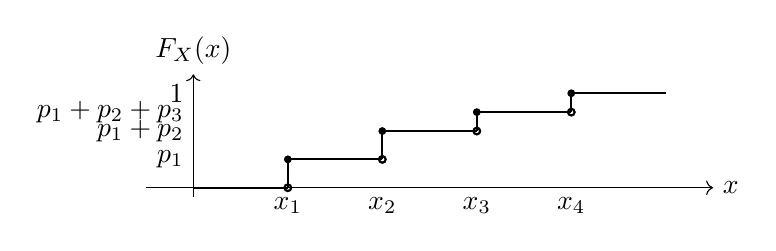
\begin{tikzpicture}[scale=1.2]
        % Assi
        \draw[->] (-0.5, 0) -- (5.5, 0) node[right] {$x$};
        \draw[->] (0, -0.1) -- (0, 1.2) node[above] {$F_X(x)$};
        
        % Punti di salto
        \draw[thick] (0, 0) -- (1, 0);
        \draw[thick] (1, 0) -- (1, 0.3);
        \draw[thick] (1, 0.3) -- (2, 0.3);
        \draw[thick] (2, 0.3) -- (2, 0.6);
        \draw[thick] (2, 0.6) -- (3, 0.6);
        \draw[thick] (3, 0.6) -- (3, 0.8);
        \draw[thick] (3, 0.8) -- (4, 0.8);
        \draw[thick] (4, 0.8) -- (4, 1);
        \draw[thick] (4, 1) -- (5, 1);
        
        % Punti
        \filldraw[black] (1, 0.3) circle (1pt);
        \filldraw[black] (2, 0.6) circle (1pt);
        \filldraw[black] (3, 0.8) circle (1pt);
        \filldraw[black] (4, 1) circle (1pt);
        
        % Cerchi vuoti
        \draw[thick] (1, 0) circle (1pt);
        \draw[thick] (2, 0.3) circle (1pt);
        \draw[thick] (3, 0.6) circle (1pt);
        \draw[thick] (4, 0.8) circle (1pt);

        % Etichette
        \node[below] at (1, 0) {$x_1$};
        \node[below] at (2, 0) {$x_2$};
        \node[below] at (3, 0) {$x_3$};
        \node[below] at (4, 0) {$x_4$};
        \node[left] at (0, 0.3) {$p_1$};
        \node[left] at (0, 0.6) {$p_1 
        + p_2$};
        \node[left] at (0, 0.8) {$p_1 + p_2 + p_3$};
        \node[left] at (0, 1) {$1$};
      \end{tikzpicture}
  \end{center}
      Quindi $ F_X $ e' data dalla formula:
      \[
        F_X(x) = \sum_{x_i \in S_X.\ x_i \leq x} p_X(x_i),\quad \forall x \in \mathbb{R}
      \]
    \item se $B$ è un sottoinsieme dei possibili valori di $X$ (anche con probabilita' nulla), allora:
  \begin{equation}
    \P(X\in B) = \P_X(B) = \sum_{x_i\in B}p_X(x) = \sum_{x_i\in B}\Delta F_X(x_i)
  \end{equation}
  \end{enumerate}
}

\ex{Esercizio Riassuntivo (2.1 libro)}{
  Sia $ G: \mathbb{R} \to [0,1] $ una funzione data da:
  \[
    G(x) = \begin{cases}
    0 & x < 0\\
    1/2 & 0\leq x < 1\\
    2/3 & 1\leq x<2\\
    11/12 & 2\leq x < 3\\
    1 & x\geq 3
    \end{cases}
  \]
  \begin{enumerate}
  \item Mostrare che $ G $ e' una funzione di ripartizione.
  \item Mostrare che $ X $ e' discreta. Determinare supporto e densita' discreta di $ X $.
  \item Trovare $ P_X $
  \item Calcolare $ P(X > 1/2), P(2 < X \leq 4), P(1< X<2), P(X < 3) $.
  \item Mostrare che $ Y = (X-2)^2 $ e' una variabile aleatoria discreta. Determinare $ S_Y e p_Y $.
  \end{enumerate}
  \textbf{Soluzione}:
  \begin{enumerate}
  \item Dobbiamo dimostrare che $ G $ ha le quattro proprieta' delle funzioni di ripartizione:
    \begin{itemize}
    \item E' ovviamente monotona crescente
    \item In tutti i punti di discontinuita', e' sempre continua a dx ($ \lim_{x\to k^{+}} G(x) = k $)
    \item I limiti a sx e dx sono 0 e 1
    \end{itemize}
    Quindi $ G $ e' una funzione di ripartizione.
    \item Essendo $ F_X(x) $ costante a tratti, $ X $ e' per forza discreta con supporto $ S_X = \{0, 1, 2, 3\} $.

      La densita' discreta $ p_X(x) $ si calcola guardando il "salto" di $ F_X(x) $ nel punto $ x $:
      \[
        \forall x \in S_X.\ p_X(x) = F_X(x) - F_X(x^{-}) = \Delta F_X(x)
      \]
      TODO: fare graficuccio e tabellonski
    \item Per la caratterizzazione della distribuzione usando la densita:
      \[
        P_X(B) = \sum_{x \in S_X} p_X(x)\delta_x(B)
      \]
    \item Va beh usa il punto prima per fare sta roba
    \item $ Y $ e' una VA che puo' essere riscritta come una composizione fra una funzione $ Z: \mathbb{R} \to \mathbb{R}.\ Z(x) = (x-2)^2 $ e $ X $. Per questo motivo, se $ X $ ha lo stesso valore per degli $ \omega \in \Omega $, allora anche in $ Y $ quegli $ \omega $ avranno la stessa immagine. Ovvero, $ |Im(Y)| \leq |Im(X)| $, che implica che $ |S_Y| \leq |S_X| $. In piu', possiamo dire che:
      \[
        p_Y(y) = \sum_{x \in Z^{-1}(y)} p_X(x) \quad \forall y \in \mathbb{R}
      \]
      Quindi $ S_Y = \{y \in \mathbb{R} | \exists x \in S_X.\ y = Z(x)\} $ TODO: molte di ste cose non le ho dimostrate/spiegate bene, forse sarebbe meglio farlo prima?
  \end{enumerate}
}
\section{Indici di sintesi di una distribuzione}

La distribuzione di una VA discreta puo' essere descritta in maniera sintetica tramite due quantita' numeriche: 
\begin{itemize}
\item La \textit{media}, che indica il valore "centrale" della distribuzione, ovvero il valore medio di $ X $ pesato con le probabilita' di ogni valore
\item La \textit{varianza}, che e' un indice di dispersione, ossia ci dice quanto quanto la distribuzione si concentra attorno alla media
\end{itemize}

\subsection{Media o valore atteso}
\dfn{Valore atteso di una variabile aleatoria}{
  Se $X$ è una variabile aleatoria discreta con densità di probabilità $p_X$, allora il valore atteso di $X$ è:
  \[
    E[X] \coloneq \sum_{x\in S_X} x p_X(x)
  \]
}
\nt{
  \begin{align*}
    \mathbb{E}[X - \mathbb{E}[X]] &= \mathbb{E}[X] - \mathbb{E}[\mathbb{E}[X]]\\
    &= \mathbb{E}[X] - \mathbb{E}[X] = 0
  \end{align*}
}
\thm{Stabilita' delle VA con composizione}{
  Sia $X$ una variabile aleatoria discreta con densità di probabilità $p_X$ e sia $g:\mathbb{R}\to \mathbb{R}$ una funzione. Allora il valore atteso di $g(X)$ è:
  \[
    \mathbb{E}[g(X)] = \sum_{x\in S_X} g(x)p_X(x)
  \]
}
\mprop{Linearita' del Valore atteso}{
  Siano $ X,Y $ VA discrete, allora $ \forall \alpha, \beta \in \mathbb{R} $:
  \[
    \mathbb{E}[\alpha \cdot X + \beta \cdot Y] = \alpha \mathbb{E}[X] + \beta \mathbb{E}[Y]
  \]
}
\pf{Dimostrazione}{
  Il bro fa una dimostrazione prendendo un solo caso, non ho capito TODO: boh
}

\subsection{Varianza}
\dfn{Varianza di $X$ }{
  Se $X$ è una variabile aleatoria discreta con densità di probabilità $p_X$ e valore atteso $E[X]$, allora la varianza di $X$ è:
  \[
    Var(X) = E[(X-E[X])^2] = \sum_{x\in S_X} (x-E[X])^2 p_X(x)
  \]
  La varianza e' anche indicata con $ \sigma^2 $.
}

\mprop{}{
  Si osservi che:
  \begin{align*}
    var(X) &= \mathbb{E}[X^2] - (\mathbb{E}[X])^2\\
    &= \sum_{x \in S_X} x^2 \cdot p_X(x) - \left( \sum_{x \in S_X} x \cdot p_X(x) \right)^2
  \end{align*}
}

\dfn{Deviazione standard}{
  Si definisce \textit{deviazione standard} la quantita':
  \[
    \sigma(X) \coloneq \sqrt{var(X)}
  \]
}
\nt{
  Se $ X $ e' una grandezza fisica espressa in una certa unita di misura, la deviazione standard ha il vantaggio di avere la stessa unita' di misura.
}
\section{Distribuzioni notevoli di VA discrete}

\subsection{Distribuzione uniforme discreta}
\dfn{Distribuzione uniforme discreta}{
  Una variabile aleatoria $X$ si dice avere una distribuzione uniforme discreta su un insieme di supporto $S_X = \{x_1, \dots, x_n\}$ di cardinalità $n$ se la densità di probabilità di $X$ è:
  \[
    p_X(x) = \frac{1}{n}, \quad \forall x\in S_X
  \]
  E si scrive $ X \sim Unif(\{x_1,...,x_n\}) $
}

Si può rappresentare questa distribuzione attraverso questa tabella:
\begin{center}
  \begin{tabular}{c|c|c|c|c|c}
    $X$ & $x_1$ & $x_2$ & $\dots$ & $x_n$ &  \\
    \hline
    $p_X(x)$ & $\frac{1}{n}$ & $\frac{1}{n}$ & $\dots$ & $\frac{1}{n}$ & 1\\ 
  \end{tabular}
\end{center}

In pratica il valore atteso di una variabile aleatoria con distribuzione uniforme discreta è:
\[
  E[X] = \sum_{x\in S_X} x p_X(x) = \sum_{x\in S_X} x \frac{1}{n} = \frac{1}{n}\sum_{x\in S_X} x = \frac{1}{n} \frac{n(n+1)}{2} = \frac{n+1}{2}
\]

mentre la varianza è:
\[
  Var(X) = \sum_{x\in S_X} (x-E[X])^2 p_X(x) = \frac{1}{n} \sum_{i=1}^n (x_i - E[X])^2
\]

\subsection{Distribuzione di Bernulli}
\dfn{Distribuzione di Bernulli di parametro $p\in [0,1]$}{
  Una variabile aleatoria $X$ con un insieme di supporto $S_X = \{ 0,1 \}$ si dice avere una distribuzione di Bernoulli di parametro $p$ se la sua densità di probabilità è:
  \[
    p_X(x) = 
    \begin{cases}
      p & \text{se } x=1,\\
      1-p & \text{se } x=0
    \end{cases}
  \]
}
Si può rappresentare questa distribuzione attraverso questa tabella:

\begin{center}
  \begin{tabular}{c|c|c|c}
    $X$ & 0 & 1& \\
    \hline
    $p_X(x)$ & $1-p$ & $p$ & 1\\ 
  \end{tabular}
\end{center}

Si noti che le variabili aleatorie di bernulli sono tutte Varaibili aleatorie indicatrici:
\[
  X = \mathbb{1}_A
\]
\[
  X(w) = \begin{cases}
    1 & w\in A\\
    0 & w\notin A
  \end{cases} \quad X \sim B(p)
\]

In pratica il valore atteso di una variabile aleatoria con distribuzione uniforme discreta è:
\[
  E[X] = \sum_{x \in S_X} x p_X(x) = 0 \cdot (1-p) + 1 \cdot p = p
\]
Mentre la sua varianza è:
\[
  Var(X) = E[X^2] - (E[X])^2 = p - p^2 = p(1-p)
\]

Si noti Inoltre che:
\[
  E[X^2] = \sum_i x_i^2 p_X (x_i) = 0 \cdot (1-p) + 1 \cdot p = p
\]

\subsection{Distribuzione binomiale di parametri $ p \in [0,1] $ e $ n \in \mathbb{N} $}
Si consideri ora una generalizzazione della distribuzione di Bernoulli, detta distribuzione binomiale. Una variabile aleatroia $X$ ha distribuzione di Bernulli sse è una variabile aleatoria indivatrice di un qualche evento $A$. Se invece consideriamo $n$ prove ripetute e indipendenti di un esperimento di Bernoulli, allora la variabile aleatoria che conta il numero di successi ottenuti in $n$ si dice che ha una distribuzione binomiale. Avremo quindi $n$ variabili aleatrie  di Bernulli:
\[
  X_1 \sim B(p), X_2\sim B(p),\dots, X_n \sim B(p)
\]
Ora si consideri la seguente variabile aleatoria:
\[
  X =\text{“n di successi negli n esperimenti”} =X_1 + X_2 + \dots + X_n
\]

Si noti questo esempio:
  \ex{Estrazione con reimmissione da un'urna}{
    Consideriamo un'urna contenente $b$ palline bianche e $r$ palline rosse, per un totale di $b + r$ palline. Si effettuano $n$ estrazioni con reimmissione, e definiamo la variabile aleatoria $X$ come:
    \[
      X = \text{``numero di palline bianche estratte''}.
    \]
    Mostrare che X `e una variabile aleatoria discreta e determinarne supporto e densità discreta.

    
  }

  \pf{Soluxione}{
    Si ha che $S_x =\{0,1,2,\dots, n\}$. Occorre calcolare $p_X(k)$ per $k = 0,1,2,\dots, n$. Sia:
    \[
      A_k = \{ X=k \}, \quad \forall k \in S_X
    \]

    l'evento si può definire:
    \[
      A_k = \{ \text{“esattamente $k$ palline bianche estratte”} \}
    \]

    Ovviamete la probabilità di $A_k$ è:
  \[
    \P(A_k) = \binom{n}{k} p^k (1-p)^{n-k}
  \]
  Dove $p= \frac{b}{b+r}$ è la probabilità di estrarre una pallina bianca in una singola estrazione.
  Quindi 
  \[
    \P(X=k) = p_X(k) = \binom{n}{k} p^k (1-p)^{n-k} \quad k = 0,1,2,\dots, n
  \]

  Come seguirà dalla definizione, $X$ ha distribuzione binomiale di parametri $n$ e $p$, ovvero $X\sim B(n,p)$

  }

Si può arrivare cisì alla definizione di distribuzione binomiale:
\dfn{}{
  Una variabile aleatoria $X$ con un insieme di supporto $S_X = \{ 0,1, \dots, n \}$ si dice avere una distribuzione binomiale di parametri $p$ e $n$ se la sua densità di probabilità è:
  \[
    p_X(x) = \binom{n}{x} p^x (1-p)^{n-x}, \quad \forall x \in S_X
  \]
}
  riassunta nella seguente tabella:
  \begin{center}
    \begin{tabular}{c|c|c|c|c|c}
      $X$ & 0 & 1 & 2 & $\dots$ & n\\
      \hline
      $p_X(x)$ & $\binom{n}{0} p^0 (1-p)^n$ & $\binom{n}{1} p^1 (1-p)^{n-1}$ & $\binom{n}{2} p^2 (1-p)^{n-2}$ & $\dots$ & $\binom{n}{n} p^n (1-p)^0$\\ 
    \end{tabular}
  \end{center}
  In tal caso scriviamo
  \[
    X\sim B(n,p)
  \]
  \nt{
    Quando $n=1$ si ha la distribuzione di Bernoulli, ovvero $B(1,p)$
  }
  \mprop{}{
    Siano$ 0 \leq p \leq 1$, $n \in N$ e $X \sim B(n, p)$. Allora
    \[
    \begin{aligned}
      E[X] &= np\\
      Var(X) &= np(1-p)
    \end{aligned}
    \]
  }
  \pf{Dimostrazione}{
    \begin{enumerate}
      \item Calcoliamo prima l'attesa $\mathbb{E}[X]$:
      \begin{align*}
      \mathbb{E}[X] &= \sum_{k=0}^n k p_X(k) = \sum_{k=1}^n k p_X(k) \\
      &= \sum_{k=1}^n k \binom{n}{k} p^k (1-p)^{n-k} \\
      &= \sum_{k=1}^n k \frac{n!}{k!(n-k)!} p^k (1-p)^{n-k} \\
      &= \sum_{k=1}^n \frac{n!}{(k-1)!(n-k)!} p^k (1-p)^{n-k} \\
      &= n p \sum_{k=1}^n \frac{(n-1)!}{(k-1)!(n-k)!} p^{k-1} (1-p)^{n-k} \\
      &\stackrel{h=k-1}{=} n p \sum_{h=0}^{n-1} \frac{(n-1)!}{h!(n-1-h)!} p^h (1-p)^{n-1-h} \\
      &\stackrel{\text{form. binom., Newton}}{=} n p.
      \end{align*}
      Qui abbiamo usato la formula del binomio e il teorema di Newton per concludere che:
      \[
      \sum_{h=0}^{n-1} \binom{n-1}{h} p^h (1-p)^{n-1-h} = 1.
      \]
      \item Calcoliamo ora la varianza $\text{Var}(X)$:
      dato che $\text{Var}(X) = \mathbb{E}[X^2] - (\mathbb{E}[X])^2$, resta da calcolare $\mathbb{E}[X^2]$. Inoltre, $\mathbb{E}[X^2] = \mathbb{E}[X(X-1)] + \mathbb{E}[X] = \mathbb{E}[X(X-1)] + np$, quindi dobbiamo calcolare $\mathbb{E}[X(X-1)]$. Si ha che:
\begin{align*}
\mathbb{E}[X(X-1)] &= \sum_{k=0}^n k(k-1) p_X(k) = \sum_{k=2}^n k(k-1) p_X(k) \\
&= \sum_{k=2}^n k(k-1) \binom{n}{k} p^k (1-p)^{n-k} \\
&= \sum_{k=2}^n k(k-1) \frac{n!}{k!(n-k)!} p^k (1-p)^{n-k} \\
&= \sum_{k=2}^n \frac{n!}{(k-2)!(n-k)!} p^k (1-p)^{n-k} \\
&= n(n-1) p^2 \sum_{k=2}^n \frac{(n-2)!}{(k-2)!(n-k)!} p^{k-2} (1-p)^{n-k} \\
&\stackrel{h=k-2}{=} n(n-1) p^2 \sum_{h=0}^{n-2} \frac{(n-2)!}{h!(n-2-h)!} p^h (1-p)^{n-2-h} \\
&\stackrel{\text{form. binom., Newton}}{=} n(n-1) p^2.
\end{align*}
Qui abbiamo nuovamente usato la formula del binomio e il teorema di Newton per concludere che:
\[
\sum_{h=0}^{n-2} \binom{n-2}{h} p^h (1-p)^{n-2-h} = 1.
\]

    \end{enumerate}
  }

\subsection{Distribuzione di Poisson}
Caso limite della distribuzione bionmiale, serve per eventi con probabilita' molto piccola. Viene passato un solo parametro $ \lambda $

\[
n\to +\infty, p\to 0, np \to \lambda > 0
\]

$ X \sim Poi(\lambda), \lambda > 0 $, $ S_X = \{0,1,...\} = \mathbb{N}_0 $ (il supporto e' infinito numerabile):
\[
  \forall k \in \mathbb{N}_0.\ p_X(k) = e^{-\lambda}\frac{\lambda^{k}}{k!}
\]

Lo sviluppo in serie di Taylor dell'esponenziale $ \forall x \in \mathbb{R} $: 
\[
\sum_{k=0}^{+\infty} \frac{x^{k}}{k!} = e^{x}
\]

\begin{align*}
  \mathbb{E}[X] &= \sum_{k=0}^{+\infty} k \frac{\lambda^{k}}{k!}e^{-\lambda} \\
  &= \lambda\sum_{k=1}^{+\infty} \frac{\lambda^{k-1}}{(k-1)!}e^{-\lambda} \\
  &= \lambda e^{-\lambda} e^{\lambda} \\
  &= \lambda \\
\end{align*}

\begin{align*}
  var(X) &= \mathbb{E}[X(X-1)] + \mathbb{E}[X] - (\mathbb{E}[X])^2\\
  &= \lambda^2 + \lambda - \lambda^2 = \lambda \\
\end{align*}

\begin{align*}
  \mathbb{E}[X(X-1)] &= \sum_{k=0}^{+\infty} k(k-1) \frac{\lambda^{k}}{k!} e^{-\lambda}\\
  &= \lambda^2 \sum_{k=1}^{+\infty} \frac{\lambda^{k-2}}{(k-2)!}e^{-\lambda} \\
  &= \lambda^2 \cdot 1 = \lambda^2 \\
\end{align*}


\section{Variabili Aleatorie Continue}

E' possibile trovarsi in una situazione in cui una variabile aleatoria puo' assumere un'infinita' \textit{continua} (e quindi non numerabile) di valori. Per questo motivo e' utile studiare le variabili aleatorie continue, che si differenziano rispetto a quelle discrete in diversi aspetti.

\ex{}{ \label{ex:VAcontTime}
  $ X = tempo di vita di un componente $

  Quindi $ X $ puo' assumere qualunque valore positivo o 0, da cui si ha
  \[  
    Im(X) = [0, +inf)
  \]

E' molto piu' naturale modellare l'intervallo di tempi come il continuo, al posto di discretizzarlo (e' una forzatura)
}

Ma, per le proprieta' del continua, questa scelta ci impone che
\[
  p_X(x) = P(X = x) = 0 \ \forall x
\]
Ovvero, le densita' discrete e' nulla per tutti i possibili valori singoli di una VA continua.

Domanda cruciale: "Come costruiamo la distribuzione di $ X $?"

Possiamo provare a calcolare la probabilita' di un intervallo di valori. Tornando all' esempio \ref{ex:VAcontTime}, ci aspettiamo che:
\[
  \forall a,b \in [0, +\infty), a < b. \quad P(a \leq X \leq b) > 0
\]
Non ci interessa quindi il valore in un punto della nostra funzione di densita', ma il valore sugli intervalli. Data una funzione $ f_X: \mathbb{R} \to \mathbb{R} $ (che chiameremo \textit{densita' continua}), possiamo provare a usare l'integrale per calcolare la probabilita' agli eventi $ \{X \in [a,b]\}  = P(a\leq X \leq b) $
\[
  P(a \leq X \leq b) = \int_{a}^{b} f_X(x)dx
\]
Notare che se $ a = b $, allora il valore dell'integrale e' nullo, proprio come ci aspettavamo. Per assicurarci che l'integrale di tale funzione sia effettivamente una proabilita', la $ f_X $ deve verificare due proprieta':
\begin{itemize}
\item Deve essere $ \geq 0 $ per ogni elemento del dominio, perche' l'integrale di una funzione negativa su un intervallo sara' sicuramente negativa
\item $ P(-\infty \leq X \leq +\infty) $ deve essere 1, dato che e' l'evento certo, quindi:
  \[
    \int_{-\infty}^{+\infty}f_X(x)dx = 1
  \]
\end{itemize}

\subsection{Definizioni di densita' e VA continue}
Diamo quindi la definizione formale di \textit{densita' continua}:
\dfn{Densita' continua}{
  Una funzione $ f_X: \mathbb{R} \to \mathbb{R} $ e' una \textit{densita' continua} se:
  \begin{itemize}
    \item $ \forall x \in \mathbb{R}.\  f(x) \geq 0 $
    \item $ \int_{+\infty}^{-\infty}f(x)dx = 1 $
  \end{itemize}
}


\ex{}{
  Un possibile valore per la densita' continua dell'esempio \ref{ex:VAcontTime}:
  \[
    f_X(x) = \begin{cases}
    0 & x<0\\
    e^{-x} & x\geq 0
    \end{cases}
  \]
  todo: graficuz

  calcola se valgono le proprieta' sopra
}

La probabilita' dell'intervallo graficamente e' l'area del sottografico di $ f_X $ nello stesso intervallo. Il vincolo e' che l'area di tutto il sottografico sia 1.

\nt{
  Notare che, a differenza della densita' discreta che ha valore massimo 1, la densita' continua non ha valore limite superiore. Cio' e' dovuto al fatto che ci interessa il suo integrale su un intervallo che non e' determinato dal valore della funzione in un solo punto, quindi puo' benissimo valere $ f_X(x) > 1 $ (puo' anche essere illimitata).
}

\ex{}{
  Nell'esempio di prima, se mettiamo $ \lambda e^{-\lambda x} $ per qualunque  l'integrale e' sempre 1!
}

Dalla definizione di densita' continua possiamo definire anche le VA continue:
\dfn{Variabile Aleatoria Continua}{
  Sia $ (\Omega, P) $ SP e $ X $ VA. Si dice che $ X $ e' \textit{continua} se $ \exists $ una densita' di probabilita', indicata con $f_X$, tale che:
  \begin{equation}
   \P(a \leq X \leq b) = \int_{a}^{b} f_X(x)dx \quad \forall [a,b] \subset \mathbb{R}
  \end{equation}
}

\ex{}{
  Esempi di utilizzo della formula:
  \begin{itemize}
    \item $ P(X \leq a) = \int_{-\infty}^{a} f_X(x)dx $
    \item $ P(X < a) = \int_{-\infty}^{a} f_X(x)dx $
    \item $ P(X > a) = \int_{a}^{+\infty} f_X(x)dx $
    \item $ P(X \in B) = \int_{B} f_X(x)dx $
    \item $ P(X \in [a,b]) = \int_{a}^{b} f_X(x)dx $
    \item $ P(X \in (a,b)) = \int_{a}^{b} f_X(x)dx $
    \item $ P(X \in [a,b)) = \int_{a}^{b} f_X(x)dx $
    \item $ P(X \in (a,b]) = \int_{a}^{b} f_X(x)dx $
    \item $ P(X \in \{a\}) = \int_{a}^{a} f_X(x)dx = 0 $
  \end{itemize}
}

\nt{
  Non esiste una sola funzione di densita' continua per una variabile. Infatti, data $ f_X $, e' possibile modificare il suo valore in un numero limitato o infinito numerabile di punti senza cambiare il valore dell'integrale:
  \[
    \forall [a,b] \subset \mathbb{R}.\quad \int_{a}^{b} f_X dx = \int_{a}^{b} g_X dx
  \]
  In questo caso, anche $ g_X $ e' una densita' di $ X $. Vedremo che cio' non causa problemi, e che in molti casi esiste una versione canonica.

  A causa di tale non unicita', non e' possibile definire un supporto, che sarebbe dato dall'insieme
  \[
    S_X = \{x \in \mathbb{R} | f_X(x) > 0\}
  \]
  dato che per diverse densita' della stessa VA gli insiemi sono diversi. Anche in questo caso possiamo considerare la densita' canonica (se c'e'), da cui deriva il supporto canonico.
}

\subsection{Funzione di Ripartizione Continua}
Una delle funzioni che ci permettono di caratterizzare le VA discrete ora diventa continua: la funzione di ripartizione (Bonzo non ci crede, e' da investigare)

Infatti, $ P(a \leq X \leq a) = P(X = a) = \int_{a}^{a}f_X(x)dx = 0 $, quindi per avere una probabilta' positiva dobbiamo per forza considerare un intervallo. Quindi, tornando alle proprieta' della funzione di ripartizione, vediamo che:
\begin{itemize}
\item $ F_X $ e' sempre continua a destra
\item $ F_X(x) - F_X(x^{-}) = P(X = x) $
\end{itemize}

Ma per quello che abbiamo detto, $ F_X $ e' continua anche a sx, quindi no more scalini.

Ebbene buon bastianini, sai come lo vedremo? GRAZIE A QUESTO EFFICACISSIMO TEOREMA:
\thm{Teorma della della densità e della continuità di $f_x$}{
  Sia $X$ una variabile aleatoria continua con densità di probabilità $f_X$. Allora:
  \begin{itemize}
    \item La densità discreta discrta di $X$ è identivamente uguale a zrto, ovvero:
    
    \[
      p_X(x) = 0 \quad \forall x \in \mathbb{R}
    \]
    \item La funzione di ripartizione $F_X$ è continua e si può calcolare come:
    \[
      F_X(x) = \int_{-\infty}^{x} f_X(y) dy
    \]
  \end{itemize}
}
\pf{Dimostrazione}{
  \begin{itemize}
    \item Dalla definizione di $p_X(x)$, abbiamo che:
    \[
      p_X(x) = P(X = x) = \int_{x}^{x} f_X(y) dy = 0
    \]
    
    Dimostrato
    \item Dalla definizione di $F_X$ si ha che 
    \[
      F_X(x) = P(X \leq x) = P(-\infty < X \leq x) = \int_{-\infty}^{x} f_X(y) dy
    \]
    Devo dimostrare che $F_X$ è contunua a destra e a sinistra:
    \begin{itemize}
      \item Devo dimostrare che $F_X$ è continua a destra, ovvero che
      
      \[
        F_X(x) = \lim_{a \to x^+} F_X(a)
      \]
      Si ha che:
      \[
        \lim_{a \to x^{+}}F_X(a) = \lim_{a \to x^{+}} \P(X \leq a) = \lim_{a \to x^{+}} \int_{-\infty}^{a} f_X(y) dy = \int_{-\infty}^{x} f_X(y) dy = F_X(x)
      \]
      Dimostrato
      \item Devo dimostrare che $F_X$ è continua a sinistra, ovvero che
      \[
        F_X(x) = \lim_{a \to x^{-}} F_X(a)
      \]
      E si ha che $\lim_{a\to x^-}F_X(a) = \P(X<x)$, allora
      \[
        \lim_{a \to x^{-}} F_X(a) = \P(X < x) = \lim_{a \to x^{-}} \int_{-\infty}^{a} f_X(y) dy = \int_{-\infty}^{x} f_X(y) dy = F_X(x)
      \]
    \end{itemize}
  \end{itemize}
}

Quindi, la funzione di ripartizione di una VA continua e' una funzione integrale, ed e' percio' \textit{assolutamente continua} (quindi e' continua con altre proprieta' in piu')

\nt{
  Si può notare quindi che:
  \[
    \P(a<X<b) = \P(a\leq X \leq b) = \P(a<X\leq b) = \P(a\leq X< b) = \int_{a}^{b} f_X(x) dx
  \]

  sono in particolare date da

  \[
    F_X (b) - F_X(a) = \int_{a}^{b} f_X(x) dx
  \]
  A differenza delle VA discrete, quindi, l'inclusione o meno degli estremi non cambia il valore della probabilita' su un intervallo.
}

\subsection{Confronto tra VA continua e discreta}
\begin{tabular}{|c|c|}
  \hline
  \textbf{Variabili aleatorie discrete} & \textbf{Variabili aleatorie continue} \\
  \hline
  densità discreta $p_X$ & densità continua $f_X$ \\
  \hline
  $\mathbb{P}(X \in B) = \sum_{x_i \in B} p_X(x_i)$ & $\mathbb{P}(X \in B) = \int_B f_X(x) \, dx$ \\
  \hline
  $F_X$ è costante a tratti: & $F_X$ è una funzione integrale o, equivalentemente, è una funzione assolutamente continua: \\
  $F_X(x) = \sum_{x_i \leq x} p_X(x_i)$ & $F_X(x) = \int_{-\infty}^x f_X(y) \, dy$ \\
  \hline
\end{tabular}

\subsection{Dalla funzione di ripartizione alla densità continua}
Dal teorema precedente sappiamo che 
\[
  F_X(x) = \int_{-\infty}^{x} f_X(y) dy
\]

Viene quindi da chiedersi come calcolare il contrario, ci dobbiamo porre quindi due domande:
\begin{itemize}
\item Che proprieta' deve avere $ F_X $ per essere sicuri che $ X $ e' continua?
\item Come si trova $ f_X $ partendo da $ F_X $?
\end{itemize}

Per rispondere alla prima domanda, sappiamo che $ X $ e' continua sse $ F_X $ e' assolutamente continua. Ma dimostrare cio' e' abbastanza difficile, quindi solitamente se non ci e' detto che $ X $ e' continua si usa tale proprieta':

\mprop{Condizione sufficente per continuita' assoluta}{
  Se una funzione $ f: \mathbb{R} \to \mathbb{R} $ e' $ C^{1} $ (differenziabile almeno una volta) a tratti, allora e' assolutamente continua
}

Dato per vero che $ X $ e' continua, dobbiamo calcolare la sua densita':

\mprop{}{
  Sia $X$ una variabile aleatoria continua con $F_X$ la sua funzione di ripartizione. Allora una densità di probabilità è data da:
  \[
    f_X(x) := \frac{d}{dx}F_X(x) \quad \forall x \text{ in cui } F_X \text{ e' derivabile}
  \]
}

\pf{Dimostrazione}{
  Sia $F_X(x)$ la funzione di ripartizione di una variabile aleatoria continua $X$. Per definizione:
  \[
    F_X(x) = \int_{-\infty}^x f_X(y) \, dy.
  \]
  Per il teorema fondamentale del calcolo integrale, se $f_X$ è continua, allora $F_X$ è derivabile e la derivata di $F_X$ è uguale alla funzione integranda $f_X$. Quindi:
  \[
    \frac{d}{dx}F_X(x) = f_X(x).
  \]
  Dimostrato.
}

\subsection{Funzioni di variabili aleatorie continue}
Siano $h: \mathbb{R} \to \mathbb{R}$ una qualunque funzione e $X$ una variabile aleatoria continua. Poniamo:
\[
  Y = h(X)
\]

Ricordiamo che quando $X$ è discreta, $Y$ è necessariamente anch’essa una variabile aleatoria discreta. Al contrario, quando X è continua, non possiamo dire nulla su $Y$ . In particolare, $Y$ potrebbe essere discreta, continua, mista. Adesso viene mostrato come calcolare la densità di probabilità di $Y$ in funzione della densità di probabilità di $X$.

\subsubsection{Metodo generale per caolare la densità di $Y$}

Per calcolare la densità di $Y$ in funzione della densità di $X$ calcolare le CDF, in pratica:
\begin{itemize}
  \item Calcolare la funzione di ripartizione $F_Y(y)$:
  \[
    F_Y (y) = P(Y \leq y) = P(h(X) \leq y) 
  \]
  \item Calcolare la densità di $Y$:
  \[
    f_Y(y) = \frac{d}{dy}F_Y(y) = \frac{d}{dy}P(h(X) \leq y)
  \]
\end{itemize}

\ex{}{
  Sia $h(x) = x^2$, quindi $Y = h(X) = X^2$. Si trovi la densità di probabilità di $Y$ in funzione della densità di probabilità di $X$.
}
\pf{Soluzione}{
  Iniziamo col determinare la funzione di ripartizione di $Y$:
  \[
    F_y (y) = P(Y \leq y) = P(X^2 \leq y) 
  \]

  Dobbiamo risolvere la disuguaglianza $X^2 \leq y$, distinguendo i due casi:
  \begin{itemize}
    \item Se $y < 0$, allora $X^2 \leq y$ non ha soluzioni, quindi $F_Y(y) = 0$.
    \item Se $y \geq 0$, allora $X^2 \leq y$ è equivalente a $-\sqrt{y} \leq X \leq \sqrt{y}$, quindi:
    \[
      F_Y(y) = P(-\sqrt{y} \leq X \leq \sqrt{y}) = P(X \leq \sqrt{y}) - P(X < -\sqrt{y}) = F_X(\sqrt{y}) - F_X(-\sqrt{y})
    \]
  \end{itemize}
  Quindi, la funzione di ripartizione di $Y$ è:
  \[
    F_Y(y) = 
    \begin{cases}
      0 & y < 0\\
      F_X(\sqrt{y}) - F_X(-\sqrt{y}) & y \geq 0
    \end{cases}
  \]
  Ora calcoliamo la densità di probabilità di $Y$:
  \[
    f_Y(y) = \frac{d}{dy}F_Y(y) = \frac{d}{dy}F_X(\sqrt{y}) - \frac{d}{dy}F_X(-\sqrt{y})
  \]
  Applicando la regola della catena, otteniamo:
  \[
    f_Y(y) = \frac{1}{2\sqrt{y}}f_X(\sqrt{y}) - \frac{1}{2\sqrt{y}}f_X(-\sqrt{y})
  \]
  Quindi, la densità di probabilità di $Y$ è:
  \[
    f_Y(y) = 
    \begin{cases}
      0 & y < 0\\
      \frac{1}{2\sqrt{y}}f_X(\sqrt{y}) - \frac{1}{2\sqrt{y}}f_X(-\sqrt{y}) & y \geq 0
    \end{cases}
  \]

}
\subsection{Distribuzioni notevoli di VA continue}
\subsubsection{Distribuzione uniforme continua}
\dfn{Distribuzione uniforme continua}{
  Una variabile aleatoria $X$ si dice avere una distribuzione uniforme continua su un intervallo $[a,b]$ se la sua densità di probabilità è:
  \begin{equation}
    f_X(x) = \frac{1}{b-a} \cdot \mathbb{1}_{(a,b)}(x) = \begin{cases}
      \frac{1}{b-a} & a \leq x \leq b\\
      0 & \text{altrimenti}
    \end{cases}
  \end{equation}
}

Si ha, quindi, che
\[
  \int_{-\infty}^{+\infty} f_X(x) dx = 1 = \int_{a}^{b} \frac{1}{b-a} dx = \frac{1}{b-a} (b-a) 
\]


Pertanto la dunzione di densità di probabilità è costante in $[a,b]$ e nulla al di fuori di questo intervallo. Si può rappresentare questa distribuzione attraverso questa tabella:
\begin{center}
  \begin{tabular}{c|c|c|c|c|c}
    $X$ & a & b & \\
    \hline
    $f_X(x)$ & $\frac{1}{b-a}$ & $\frac{1}{b-a}$ & 1\\ 
  \end{tabular}
\end{center}
Il grafico della distribuzione è il seguente: TODO: non compila
% \begin{tikzpicture}
%   \begin{axis}[
%       xlabel={$x$}, ylabel={$f_X(x)$},
%       xmin=-0.5, xmax=6,
%       ymin=-0.2, ymax=1.5,
%       axis lines=middle,
%       xticklabel style={anchor=north}, % Align x-axis labels properly
%       enlargelimits=true,
%       grid=both,
%       grid style={line width=.1pt, draw=gray!10},
%       major grid style={line width=.2pt,draw=gray!50},
%       minor tick num=4,
%       width=10cm, height=6cm,
%       domain=0:6, samples=100,
%       restrict y to domain=-0.2:1.5,
%       legend pos=north east
%   ]
%       % Plot the exponential function
%       \addplot[blue, thick] {exp(-x)} node [pos=0.9, above right] {$f_X(x) = \lambda e^{-\lambda x}$};
%      
%       % Add axis labels and annotations
%       \node at (axis cs:1,-0.2) [below] {$1$};
%       \node at (axis cs:3,-0.2) [below] {$3$};
%       \node at (axis cs:-0.2,1) [left] {$\lambda$};
%      
%       % Highlight the area under the curve
%       \addplot[blue!20] fill between[of=A and B, soft clip={domain=0:6}];
%   \end{axis}
% \end{tikzpicture}

Si possono fare ulteriori considerazioni:
\mprop{Fuznione di ripartizione di una variabile aleatoria continua con distribuzione costante}{
  Sia $X$ una variabile aleatoria continua con distribuzione uniforme continua su $[a,b]$. Allora la funzione di ripartizione di $X$ è:
  \[
    F_X(x) = 
    \begin{cases}
      0 & x < a\\
      \frac{x-a}{b-a} & a \leq x \leq b\\
      1 & x > b
    \end{cases}
  \]
  }
  \nt{
    Si noti che la funzione di ripartizione è continua e crescente in $[a,b]$.
  }
  \pf{Dimostrazione}{
    La funzione di ripartizione è definita come:
    \[
      F_X(x) = P(X \leq x) = \int_{-\infty}^{x} f_X(y) dy
    \]
    Quindi, per calcolare la funzione di ripartizione, dobbiamo considerare i tre casi:
    \begin{itemize}
      \item Se $x < a$, allora $F_X(x) = 0$.
      \item Se $a \leq x \leq b$, allora:
      \[
         F_X(x) = \int_{-\infty}^{x} f_X(y) dy = \int_{a}^{x} f_X(y) dy = \int_{a}^{x} \frac{1}{b-a} dy = \frac{x-a}{b-a}
      \]
      \item Se $x > b$, allora $F_X(x) = 1$
    \end{itemize}
  }


Ora passiamo a calcolare il valore atteso e la varianza di una variabile aleatoria continua con distribuzione uniforme continua:
\mprop{}{
  Sia $X$ una variabile aleatoria continua con distribuzione uniforme continua su $[a,b]$. Allora:
  \[
    E[X] = \frac{a+b}{2}
  \]
  \[
    Var(X) = \frac{(b-a)^2}{12}
  \]
}
\pf{Dimostrazione}{
  Ricordando che
  \[
    f_X(x) =\frac{1}{b-a}
  \]
  \begin{align*}
    E[X] &= \int_{-\infty}^{+\infty} x f_X(x) dx = \int_{a}^{b} x \frac{1}{b-a} dx = \frac{1}{b-a} \left[ \frac{x^2}{2} \right]_{a}^{b} = \frac{1}{b-a} \left( \frac{b^2}{2} - \frac{a^2}{2} \right)\\
    &= \frac{1}{b-a} \cdot \frac{(b-a)(b+a)}{2} = \frac{a+b}{2}
  \end{align*}
  Quindi, il valore atteso di una variabile aleatoria continua con distribuzione uniforme continua su $[a,b]$ è:
  \[
    E[X] = \frac{a+b}{2}
  \]
  Per calcolare la varianza, utilizziamo la formula:
  \[
    Var(X) = E[X^2] - (E[X])^2
  \]
  Calcoliamo prima $E[X^2]$:
  \begin{align*}
    E[X^2] &= \int_{-\infty}^{+\infty} x^2 f_X(x) dx = \int_{a}^{b} x^2 f_X(x) dx = \int_{a}^{b} x^2 \frac{1}{b-a} dx\\
    &= \frac{1}{b-a} \left[ \frac{x^3}{3} \right]_{a}^{b} = \frac{1}{b-a} \left( \frac{b^3}{3} - \frac{a^3}{3} \right)\\
    &=\frac{1}{3(b-a)} (b^3 - a^3) =\frac{(b-a)(b^2 + ab + a^2)}{3(b-a)}\\
    &=\frac{(b^2 + ab + a^2)}{3}
  \end{align*}
  Quindi, la varianza è:
  \begin{align*}
    Var(X) &= E[X^2] - (E[X])^2 = \frac{(b^2 + ab + a^2)}{3} - \left( \frac{a+b}{2} \right)^2\\
    &= \frac{(b^2 + ab + a^2)}{3} - \frac{(a^2 + 2ab + b^2)}{4}\\
    &= \frac{4(b^2 + ab + a^2) - 3(a^2 + 2ab + b^2)}{12}\\
    &= \frac{(b^2 - 2ab + a^2)}{12} = \frac{(b-a)^2}{12}
  \end{align*}
}

\subsubsection{Distribuzione esponenziale}

La distribuzione esponenziale si ha quando si ha un processo di Poisson, ovvero quando si ha un evento che accade in un certo intervallo di tempo, ad esempio si usa per descrivere il tempo di vita di un macchinario oppure di un componente elettronico
\dfn{Distribuzione esponenziale}{
  Una variabile aleatoria $X$ si dice avere una distribuzione esponenziale con parametro $\lambda > 0$ se la sua densità di probabilità è: TODO: non compila plot
  \[
    f_X(x) = \lambda e^{-\lambda x} \cdot \mathbb{1}_{(0,+\infty)}(x) = \begin{cases}
      \lambda e^{-\lambda x} & x \geq 0\\
      0 & \text{altrimenti}
    \end{cases}
      % \addplot[blue, thick, name path=A] {\lambda * exp(-\lambda * x)} node [pos=0.9, above right] {$f_X(x)$};
  \]
}

il cui grafico è: TODO
% \begin{tikzpicture}
%   \begin{axis}[
%       xlabel={$x$},
%       ylabel={$f_X(x)$},
%       xmin=-0.5, xmax=6,
%       ymin=-0.2, ymax=1.5,
%       axis lines=middle,
%       enlargelimits=true,
%       grid=both,
%       grid style={line width=.1pt, draw=gray!10},
%       major grid style={line width=.2pt,draw=gray!50},
%       minor tick num=4,
%       width=10cm,
%       height=6cm,
%       domain=0:6,
%       samples=100,
%       restrict y to domain=-0.2:1.5,
%       legend pos=north west,
%       xtick=\empty, % Rimuove le etichette sull'asse x
%       ytick=\empty  % Rimuove le etichette sull'asse y
%   ]
      
%       % Disegna la funzione esponenziale
%       \addplot[blue, thick, name path=A] {exp(-x)} node [pos=0.9, above right] {$f_X(x)$};
      
%       % Riempi l'area sotto la curva
%       \addplot[blue!20] fill between[of=A and B, soft clip={domain=0:6}];
      
%       % Linee tratteggiate verticali
%       \draw[dashed] (axis cs:1,0) -- (axis cs:1,{exp(-1)});
%       \draw[dashed] (axis cs:3,0) -- (axis cs:3,{exp(-3)});
      
%       % Etichette degli assi
%       \node at (axis cs:1,-0.2) [below] {$a$};
%       \node at (axis cs:3,-0.2) [below] {$b$};
%       \node at (axis cs:-0.2,1) [left] {$\lambda$};
      
%       % Aggiungi legenda
%       \addlegendentry{Area sotto la curva: $P(a \leq X \leq b)$}
      
%       % Asse x
%       \addplot[black, thick, name path=B] {0};
%   \end{axis}
% \end{tikzpicture}


Si noti che
\mprop{Funzione di ripartizione di una variabile aleatoria continua con distribuzione esponenziale}{
  Sia $X$ una variabile aleatoria continua con distribuzione esponenziale con parametro $\lambda > 0$. Allora la funzione di ripartizione di $X$ è:
  \begin{equation} 
    F_X(x) = 
    \begin{cases}
      0 & x < 0\\
      1 - e^{-\lambda x} & x \geq 0
    \end{cases}  
  \end{equation}
  In tal caso scriviamo
  \[
    X \sim \text{Exp}(\lambda)
  \]
}
\pf{Dimostrazione}{
  La funzione di ripartizione è definita come:
  \[
    F_X(x) = P(X \leq x) = \int_{-\infty}^{x} f_X(y) dy
  \]
  Quindi, per calcolare la funzione di ripartizione, dobbiamo considerare i due casi:
  \begin{itemize}
    \item Se $x < 0$, allora $F_X(x) = 0$.
    \item Se $x \geq 0$, allora:
    \[
      F_X(x) = \int_{-\infty}^{x} f_X(y) dy = \int_{0}^{x} f_X(y) dy = \int_{0}^{x} \lambda e^{-\lambda y} dy = -e^{-\lambda y} \bigg|_0^x = -e^{-\lambda x} + 1
    \]
    Quindi, la funzione di ripartizione di $X$ è:
    \[
      F_X(x) = 
      \begin{cases}
        0 & x < 0\\
        1 - e^{-\lambda x} & x \geq 0
      \end{cases}
    \]
  \end{itemize}
}

\nt{
  Si noti che la funzione di ripartizione è continua e crescente in $[0,+\infty)$.
}

\mprop{}{
  Sia $X$ una variabile aleatoria continua con distribuzione esponenziale con parametro $\lambda > 0$. Allora:
  \[
    E[X] = \frac{1}{\lambda}
  \]
  \[
    Var(X) = \frac{1}{\lambda^2}
  \]
}
\pf{Dimostrazione}{
  Ricordando che
  \[
    f_X(x) = \lambda e^{-\lambda x}
  \]
  \begin{align*}
    E[X] &= \int_{-\infty}^{+\infty} x f_X(x) dx = \int_{0}^{+\infty} x \lambda e^{-\lambda x} dx\\
    &= -\frac{1}{\lambda^2} e^{-\lambda x} (x + \frac{1}{\lambda}) \bigg|_0^{+\infty}\\
    &= -\frac{1}{\lambda^2} (0 + 0) + \frac{1}{\lambda^2} = \frac{1}{\lambda}
  \end{align*}
  Quindi, il valore atteso di una variabile aleatoria continua con distribuzione esponenziale è:
  \[
    E[X] = \frac{1}{\lambda}
  \]
  Per calcolare la varianza, utilizziamo la formula:
  \[
    Var(X) = E[X^2] - (E[X])^2
  \]
  Calcoliamo prima $E[X^2]$:
  \begin{align*}
    E[X^2] &= \int_{-\infty}^{+\infty} x^2 f_X(x) dx = \int_{0}^{+\infty} x^2 \lambda e^{-\lambda x} dx\\
    &= -\frac{1}{\lambda^3} e^{-\lambda x} (x^2 + 2\frac{x}{\lambda} + \frac{1}{\lambda^2}) \bigg|_0^{+\infty}\\
    &= -\frac{1}{\lambda^3} (0 + 0 + 0) + \frac{1}{\lambda^3} = \frac{2}{\lambda^2}
  \end{align*}
  Quindi, la varianza è:
  \begin{align*}
    Var(X) &= E[X^2] - (E[X])^2 = \frac{2}{\lambda^2} - \left( \frac{1}{\lambda} \right)^2\\
    &= \frac{2}{\lambda^2} - \frac{1}{\lambda^2} = \frac{1}{\lambda^2}
  \end{align*}
}

\nt{
  Si noti che la varianza è sempre positiva e tende a zero quando $\lambda$ tende a infinito.
}

\subsubsection{
  Distribuzione Normale (o Gaussiana)
}
\dfn{Distribuzione Normale}{
  Una variabile aleatoria $X$ si dice avere una distribuzione normale con media $\mu \in \mathbb{R}$ e varianza $\sigma^2 > 0$ se la sua densità di probabilità è:
  \[
    f_X(x) = \frac{1}{\sqrt{2\pi\sigma^2}} e^{-\frac{(x - \mu)^2}{2\sigma^2}}
  \]
  in tal caso scriviamo
  \[
    X \sim \mathcal{N}(\mu, \sigma^2)
  \]
}
Qui la sua funzione di ripartizione è
\mprop{
  Funzione di ripartizione di una variabile aleatoria continua con distribuzione normale}{
  Sia $X$ una variabile aleatoria continua con distribuzione normale con media $\mu \in \mathbb{R}$ e varianza $\sigma^2 > 0$. Allora la funzione di ripartizione di $X$ è:
  \[
    F_X(x)= \frac{1}{2} \left( 1 + \text{erf}\left( \frac{x - \mu}{\sigma\sqrt{2}} \right) \right)
  \]
}
\pf{Dimostrazione}{
  La funzione di ripartizione è definita come:
  \[
    F_X(x) = P(X \leq x) = \int_{-\infty}^{x} f_X(y) dy
  \]
  Quindi, per calcolare la funzione di ripartizione, dobbiamo considerare i due casi:
  \begin{itemize}
    \item Se $x < -\infty$, allora $F_X(x) = 0$.
    \item Se $x > +\infty$, allora $F_X(x) = 1$.
    \item Se $-\infty < x < +\infty$, allora:
    \[
      F_X(x) = \int_{-\infty}^{x} f_X(y) dy = \int_{-\infty}^{x} \frac{1}{\sqrt{2\pi\sigma^2}} e^{-\frac{(y - \mu)^2}{2\sigma^2}} dy
    \]
    Questa integrale non ha una soluzione analitica, ma può essere calcolato numericamente utilizzando la funzione errore $\text{erf}$.
  \end{itemize}
}

\subsubsection{Distribuzione Normale standard}
La distribuzione normale standard è un caso particolare della distribuzione normale in cui:
\begin{itemize}
  \item La media $\mu=0$
  \item La varianza $\sigma^2=1$
\end{itemize}
La notazione è
\[
  Z \sim \mathcal{N}(0, 1)
\]
Per dovere di cronaca riporto la definizione
\dfn{Distribuzione Normale standard}{
  Una variabile aleatoria $Z$ si dice avere una distribuzione normale standard se la sua densità di probabilità è:
  \[
    \varphi_X(x) = \frac{1}{\sqrt{2\pi}} e^{-\frac{x^2}{2}}
  \]
  in tal caso scriviamo
  \[
    Z \sim \mathcal{N}(0, 1)
  \]
}

Si noti che la distribuzione normale standard è simmetrica rispetto all'asse $y$ e ha una forma a campana
\begin{center}
  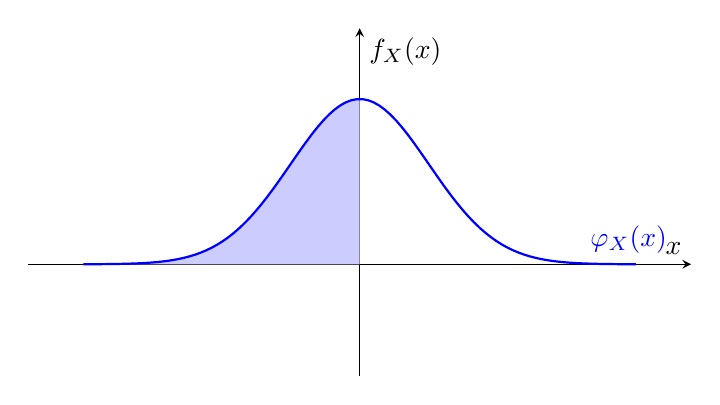
\begin{tikzpicture}
    \begin{axis}[
      xlabel={$x$},
      ylabel={$f_X(x)$},
      xmin=-4, xmax=4,
      ymin=-0.2, ymax=0.5,
      axis lines=middle,
      enlargelimits=true,
      grid=both,
      grid style={line width=.1pt, draw=gray!10},
      major grid style={line width=.2pt,draw=gray!50},
      minor tick num=4,
      width=10cm,
      height=6cm,
      domain=-4:4,
      samples=100,
      restrict y to domain=-0.2:0.5,
      xtick=\empty, % Rimuove le etichette sugli assi x
      ytick=\empty  % Rimuove le etichette sugli assi y
  ]
      
      % Disegna la distribuzione normale standard
      \addplot[blue, thick, name path=A] {1/sqrt(2*pi) * exp(-x^2/2)} node [pos=0.9, above right] {$\varphi_X(x)$};
      
      % Asse x (per il riempimento)
      \addplot[draw=none, name path=B] {0};
      
      % Riempi l'area sotto la curva
      \addplot[blue!20] fill between[of=A and B, soft clip={domain=-4:0}];
      
  \end{axis}
\end{tikzpicture}
\end{center}

Si noti la funzione di ripartizione
\mprop{funzione di ripartizione della distribuzione normale standard}{
  Sia $Z$ una variabile aleatoria continua con distribuzione normale standard. Allora la funzione di ripartizione di $Z$ è:
  \[
    F_Z(z) = \frac{1}{2} \left( 1 + \text{erf}\left( \frac{z}{\sqrt{2}} \right) \right)
  \]
}
\pf{Dimostrazione}{
  La funzione di ripartizione è definita come:
  \[
    \Phi_Z(x) = P(Z \leq z) = \int_{-\infty}^{z} f_Z(y) dy
  \]
  Quindi, per calcolare la funzione di ripartizione, dobbiamo considerare i due casi:
  \begin{itemize}
    \item Se $z < -\infty$, allora $F_Z(z) = 0$.
    \item Se $z > +\infty$, allora $F_Z(z) = 1$.
    \item Se $-\infty < z < +\infty$, allora:
    \[
      F_Z(z) = \int_{-\infty}^{z} f_Z(y) dy = \int_{-\infty}^{z} \frac{1}{\sqrt{2\pi}} e^{-\frac{y^2}{2}} dy
    \]
    Questa integrale non ha una soluzione analitica, ma può essere calcolato numericamente utilizzando la funzione errore $\text{erf}$.
  \end{itemize}
}

Questo è il grafico della funzione di ripartizione della distribuzione normale standard: TODO (non c'ho voglia di farlo ora)

Proposizione utilina
\mprop{}{
  Sia $X$ una variabile aleatoria continua con distribuzione normale standard $Z \sim \mathcal{N}(0, 1)$. Allora:
  \[
    E[Z] = 0
  \]  
  \[
    Var(Z) = 1
  \]
}
\pf{Dimostrazione}
{
  Ricordando che
  \[
    f_Z(z) = \frac{1}{\sqrt{2\pi}} e^{-\frac{z^2}{2}}
  \]
  Si ha:
  \begin{align*}
    E[Z] &= \int_{-\infty}^{+\infty} z f_Z(z) dz = \int_{-\infty}^{+\infty} z \frac{1}{\sqrt{2\pi}} e^{-\frac{z^2}{2}} dz\\
    &= 0
  \end{align*}
  Quindi, il valore atteso di una variabile aleatoria continua con distribuzione normale standard è:
  \[
    E[Z] = 0
  \]
  Per calcolare la varianza, utilizziamo la formula:
  \[
    Var(Z) = E[Z^2] - (E[Z])^2
  \]
  Calcoliamo prima $E[Z^2]$:
  \begin{align*}
    E[Z^2] &= \int_{-\infty}^{+\infty} z^2 f_Z(z) dz = \int_{-\infty}^{+\infty} z^2 \frac{1}{\sqrt{2\pi}} e^{-\frac{z^2}{2}} dz\\
    &= 1
  \end{align*}
  Quindi, la varianza è:
  \begin{align*}
    Var(Z) &= E[Z^2] - (E[Z])^2 = 1 - 0 = 1  \end{align*}
}

Adesso vengono qui riportate alcune proprietà della distribuzione normale
\mprop{}{
  Se $X \sim \mathcal{N}(\mu, \sigma^2)$, allora la trasformazione
  \[
    Z = \frac{X - \mu}{\sigma}
  \]
  è una variabile aleatoria standardizzata, ovvero $Z \sim \mathcal{N}(0, 1)$ 
}
\pf{Dimostrazione}{
  Sia $X \sim \mathcal{N}(\mu, \sigma^2)$, quindi la funzione di densità di probabilità di $X$ è:
  \[
    f_X(x) = \frac{1}{\sqrt{2\pi\sigma^2}} e^{-\frac{(x - \mu)^2}{2\sigma^2}}
  \]
  Devo dimostrare che $Z = \frac{X - \mu}{\sigma}$ ha una distribuzione normale standard, quindi:
  \[
    f_Z(z) = \frac{1}{\sqrt{2\pi}} e^{-\frac{z^2}{2}}
  \]
  Si ha che la dunzione di ripartizione di $Z$ è:
  \[
    F_Z(z) = P(Z \leq z) = P\left( \frac{X - \mu}{\sigma} \leq z \right) = P(X \leq z\sigma + \mu) = F_X(z\sigma + \mu)
  \]
  Dove $F_X(x)$ è la funzione di ripartizione di $X$.

  Per trovare la funzione di densità di probabilità di $Z$, deriviamo $F_Z(z)$ rispetto a $z$:
  \[
    f_Z(z) = \frac{d}{dz}F_Z(z) = \frac{d}{dz}F_X(z\sigma + \mu) = f_X(z\sigma + \mu) \cdot \sigma
  \]
  Sostituendo $f_X(x)$, otteniamo:
  \[
    f_Z(z) =f_X(z\sigma +\mu) = \frac{1}{\sqrt{2\pi\sigma^2}} e^{-\frac{(z\sigma + \mu - \mu)^2}{2\sigma^2}} \cdot \sigma = \frac{1}{\sqrt{2\pi}} e^{-\frac{z^2}{2}}
  \]
  
  Questo dimostra che $Z$ ha una distribuzione normale standard
}

\chapter{Integrale di Gauss}
perché sì

\[
  \int_{-\infty}^{+\infty} e^{-x^2} dx = \sqrt{\pi}
\]

\include{paginette/vettori-aleatori}
% \begin{document}
\chapter{Catene di Markov !WIP!}
Lavoriamo ancora con successioni di VA - ovvero un processo stocastico (che puo' esere a tempo discreto o continuo, dato che l'interpretazione tipica e' che gli esperimenti vengono fatti in successione nel tempo) 

$ (X_n)_{n \in \mathbb{N}} $ sono VA discrete:
\begin{itemize}
\item $ X_1 \to S_{X_1} $
\item $ X_1 \to S_{X_1} $
\item $ X_1 \to S_{X_1} $
\item $ X_1 \to S_{X_1} $
\end{itemize}

Dove tutti i supporti sono finiti o infiniti numerabili tali per cui $ \exists S  $ supporto finito o infinito numerabile che:
\[
S_{X_1} \subseteq S, ..., S_{X_i} \subseteq S
\]
\dfn{}{
  $ (X_n)_{n \in \mathbb{N}} $ di VA discrete e' detta \textit{catena di Markov} (a tempo discreto) se:
  \begin{itemize}
  \item $ \exists S  $ finito o inf. numerabile che contiene tutti i supporti
  \item Vale la proprieta' di Markov:
    \[
    \forall i, j, i
    \]
  \end{itemize}

  la i e' il valore presente mentre la j e' il valore futuro, in pratica il valore del prossimo stato e' condizionato solo dall'ultimo valore e non da quelli prima
}

in realta noi lavoreremo nel caso di $ S  $ finito, questa e' un'ipotesi innocua perche' e' facile passare alla versione infinita

la seconda non e' innocua, ci dice che ci sara' solo una matrice di transizione e il tempo non gioca nessun ruolo, quindi sapendo il valore attuale sappiamo le probabilita' di trovarci nelgi altri stati possibili il prossimo tempo

la somma delle righe della matrice deve fare 1 dato che sono tutte le possibilita'

ci possiamo porre la domanda: ora mi trovo in un punto, qual'e' la probabilita' che fra x passi mi trovi in un altro specifico punto

abbiamo visto poi un paio di esempi con grafi

che cosa si aspetta di vedere negli esercizi d'esame: formule! non numeri a caso. Sulle catene di Markov possiamo lavorare sul grafo (anche per determinare le classi di comunicazione) ma bisogna che sul grafo ci sia un segno che fa vedere il ragionamento (e' cosi in generale per tutto il compito)

classifichiamo gli stati in base al livello di accessibilita'. 

Legge delle VA data la matrice delle probabilita' di transizione

queste dipendono dal tempo e dalla distribuzione dello stato di partenza, anche se in realta' non deve essere per forza il primo stato, basta uno qualunque perche' tanto ci interessa solo dello stato finale. Quindi se viene dato il penultimo stato ci basta guardare un solo passaggio (e' meglio!)

% \end{document}

% \begin{document}
\chapter{Esercitazione}
\section{Probabilita' Condizionata}
\subsection{Esercizio 4 (Foglio 2)}
\subsubsection{Testo}
Un’urna contiene \(r\) palline rosse e \(b\) palline bianche. Si eseguono due estrazioni senza reimmissione.
\begin{enumerate}[label=(\alph*)]
    \item Determinare uno spazio di probabilità che descriva l’esperimento aleatorio.
    \item Calcolare la probabilità che la prima pallina estratta sia rossa.
    \item Calcolare la probabilità che la prima pallina sia rossa e la seconda bianca.
    \item Calcolare la probabilità che le due palline abbiano colori diversi.
    \item Calcolare la probabilità che la seconda pallina estratta sia rossa.
\end{enumerate}

\subsubsection{Soluzione}
Siano:

$R_i$ = "ho estratto una pallina rossa all'i-esima iterazione"
$B_i$ = "ho estratto una pallina rossa all'i-esima iterazione"

Definiamo lo spazio degli esiti. Poiché le estrazioni avvengono senza reimmissione, ogni esito è una coppia ordinata di palline diverse. Denotiamo:
\[
    \Omega = \{ (p_1, p_2) : p_1, p_2 \text{ sono palline dell'urna e } p_1 \neq p_2 \}
\]
La cardinalità totale è:
\[
    |\Omega| = (r+b)(r+b-1)
\]
Infatti appena estraiamo una pallina l'urna conterrà $(r+b-1)$ palline, la totalità di palline -1

Sfruttiamo il principio di probabilità uniforme, secondo cui ogni esito ha probabilità \(1/|\Omega|\)

\begin{enumerate}[label=(\alph*)]
    \item \textbf{Spazio di probabilità:}\\
    Lo spazio di probabilità è \((\Omega, P)\) con
    \[
        P(\{ \omega \}) = \frac{1}{(r+b)(r+b-1)} \quad \forall \omega \in \Omega.
    \]
    
    \item \textbf{Probabilità che la prima pallina sia rossa:}\\[1mm]
    Poiché ci sono \(r\) palline rosse su un totale di \(r+b\), si ha:
    \[
        P(R_1) = \frac{r}{r+b}.
    \]
    
    \item \textbf{Probabilità che la prima pallina sia rossa e la seconda bianca:}\\[1mm]
    Dato che la prima è rossa, nell’urna rimangono \(r+b-1\) palline, di cui \(b\) sono bianche:
    \[
        P(R_1 \cap B_2) = P(B_2 | R_1) P(R_1) =\frac{r}{r+b} \cdot \frac{b}{r+b-1}.
    \]
    
    \item \textbf{Probabilità che le due palline abbiano colori diversi:}\\[1mm]
    Questa condizione si verifica in due modi: rossa poi bianca oppure bianca poi rossa. Quindi:
    \[
        \begin{split}
            P((R_1 \cap B_2)\cup (B_1 \cap R_2)) & =P(B_2 | R_1) P(R_1) + P(R_2 | B_1) P(B_1)\\
                    &= \frac{r}{r+b} \cdot \frac{b}{r+b-1} + \frac{b}{r+b} \cdot \frac{r}{r+b-1} \\
                    &= \frac{2rb}{(r+b)(r+b-1)}.
        \end{split}
    \]
    \item \textbf{Probabilità che la seconda pallina sia rossa:}\\[1mm]
    Usiamo la formula della probabilità totale, considerando le possibili estrazioni del primo turno:
    \[
    \begin{split}
    P(R_2) &= P(B_2 \mid R_1) \cdot P(R_1)  + P(B_2 \mid B_1) \cdot P(B_1)\\[1mm]
    &= \frac{r-1}{r+b-1} \cdot \frac{r}{r+b} + \frac{r}{r+b-1} \cdot \frac{b}{r+b}
    \end{split}
    \]
    Semplificando:
    \[
    P(R_2) = \frac{r(r-1) + rb}{(r+b)(r+b-1)} = \frac{r^2 - r + rb}{(r+b)(r+b-1)} = \frac{r(r+b-1)}{(r+b)(r+b-1)} = \frac{r}{r+b}
    \]
\end{enumerate}

\subsubsection{Esercizio 6}
\subsubsection{Testo}
Supponiamo che un’urna contenga 1 pallina rossa e 1 pallina bianca. Una pallina viene estratta e se ne osserva il colore. La pallina estratta viene poi rimessa nell’urna insieme a un’altra pallina dello stesso colore (estrazione con rinforzo). Siano
\[
\begin{aligned}
    R_i &= \text{evento che all'}i\text{-esima estrazione venga estratta una pallina rossa,}\\
    B_i &= \text{evento che all'}i\text{-esima estrazione venga estratta una pallina bianca.}
\end{aligned}
\]
Si calcolino:
\begin{enumerate}[label=(\arabic*)]
    \item \(P(R_2)\)
    \item Sapendo che la seconda pallina estratta è rossa, quale è l’evento più probabile per la prima estrazione: che la pallina estratta sia stata rossa oppure bianca?
\end{enumerate}

\subsubsection{Soluzione}
\begin{enumerate}[label=(\arabic*)]
    \item \textbf{Calcolo di \(P(R_2)\):}\\[1mm]
    \textbf{Caso 1:} Se alla prima estrazione esce una pallina rossa (evento \(R_1\)):
    \begin{itemize}
        \item La probabilità di estrarre una rossa al primo turno è \(P(R_1)=\frac{1}{2}\).
        \item Dopo l’estrazione, la pallina rossa viene rimessa insieme a un’altra rossa, dunque l’urna contiene 2 rosse e 1 bianca. Quindi:
        \[
        P(R_2 \mid R_1)=\frac{2}{3}.
        \]
    \end{itemize}
    \textbf{Caso 2:} Se alla prima estrazione esce una pallina bianca (evento \(B_1\)):
    \begin{itemize}
        \item \(P(B_1)=\frac{1}{2}\).
        \item Dopo il rinforzo, l’urna contiene 1 rossa e 2 bianche, dunque:
        \[
        P(R_2 \mid B_1)=\frac{1}{3}.
        \]
    \end{itemize}
    Applicando la formula della probabilità totale:
    \[
    \begin{split}
    P(R_2) &= P(R_2 \mid R_1) \cdot P(R_1) + P(R_2 \mid B_1) \cdot P(B_1) \\
    &= \frac{2}{3}\cdot\frac{1}{2} + \frac{1}{3}\cdot\frac{1}{2} \\
    &= \frac{1}{3} + \frac{1}{6} = \frac{1}{2}.
    \end{split}
    \]
    
    \item \textbf{Confronto tra \(P(R_1 \mid R_2)\) e \(P(B_1 \mid R_2)\):}\\[1mm]
    
    Innanzi tutto si tenga conto il teorema di Bayes:\\ 
    Siano $A,B$ due eventi, t.c. $P(A), P(B)>0$, allora $P(A\mid B) = \frac{P(B\mid A) P(A)}{P(B)}$

    Dimostrazione: 
    Abbiamo $P(A\cap B) = P(B\cap A)$, quindi $P(A\mid B) = \frac{P(A\cap B)}{P(B)} = \frac{P(B\mid A)P(A)}{P(B)}$


    Usiamo il teorema di Bayes per calcolare \(P(R_1 \mid R_2)\):
    \[
    P(R_1 \mid R_2) = \frac{P(R_2 \mid R_1) \, P(R_1)}{P(R_2)} 
    = \frac{\frac{2}{3} \cdot \frac{1}{2}}{\frac{1}{2}}
    = \frac{2}{3}.
    \]
    Poiché \(P(B_1 \mid R_2) =1- P(B_1^c \mid R_2) =1 - P(R_1 \mid R_2) = 1 - \frac{2}{3} = \frac{1}{3}\), risulta che,
    \[
    P(R_1 \mid R_2) > P(B_1 \mid R_2).
    \]
    Quindi, sapendo che la seconda pallina è rossa, è più probabile che la prima pallina estratta fosse rossa.
\end{enumerate}


\subsection{Esercizio 7}
\subsubsection{Testo}
Si consideri una popolazione in cui una persona su 100 abbia una certa malattia. Un test è disponibile per diagnosticare tale malattia. Si supponga che il test non sia perfetto, in quanto esso risulta positivo (ovvero indica la presenza della malattia) nel 5\% dei casi quando è effettuato su persone sane, mentre risulta negativo (indicando l’assenza della malattia) nel 2\% dei casi quando è effettuato su persone malate. Si calcolino le probabilità che:
\begin{enumerate}[label=(\alph*)]
    \item il test risulti positivo quando effettuato su una persona malata,
    \item il test risulti positivo,
    \item una persona sia malata se il test risulta positivo.
\end{enumerate}

\subsubsection{Soluzione}
I dati del problema sono: 
\begin{itemize}
    \item \(P(M)=0.01\): probabilità che una persona sia malata.
    \item \(P(S)=0.99\): probabilità che una persona sia sana.
    \item \(P(T^+ \mid M)=0.98\): probabilità che il test risulti positivo se la persona è malata.
    \item \(P(T^- \mid M)=0.02\): probabilità che il test risulti negativo se la persona è malata.
    \item \(P(T^+ \mid S)=0.05\): probabilità che il test risulti positivo se la persona è sana.
    \item \(P(T^- \mid S)=0.95\): probabilità che il test risulti negativo se la persona è sana.
\end{itemize}


Costruiamo un diagramma di verità:
\begin{center}
    \begin{tabular}{|c|c|c|}
        \hline
        & Malato & Sano \\
        \hline
        Positivo & 0.98 & 0.05 \\
        \hline
        Negativo & 0.02 & 0.95 \\
        \hline
    \end{tabular}
\end{center}


\begin{enumerate}
    \item \textbf{Probabilità che il test risulti positivo su una persona malata}: Questa probabilità è data direttamente dai dati:
    \[
        P(T^+ \mid M)=0.98.
    \]
    
    \item \textbf{Probabilità che il test risulti positivo}:Utilizziamo la formula della probabilità totale:
    \[
    \begin{split}
    P(T^+) &= P(T^+ \mid M) \, P(M) + P(T^+ \mid S) \, P(S) \\
    &= 0.98 \cdot 0.01 + 0.05 \cdot 0.99 \\
    &= 0.0098 + 0.0495 \\
    &\approx 0.0593.
    \end{split}
    \]
    
    \item \textbf{Probabilità che una persona sia malata, dato un test positivo:}\\[1mm]
    Applichiamo il teorema di Bayes:
    \[
    \begin{split}
    P(M \mid T^+) &= \frac{P(T^+ \mid M) \, P(M)}{P(T^+)} \\
    &= \frac{0.98 \cdot 0.01}{0.0593} \\
    &\approx \frac{0.0098}{0.0593} \\
    &\approx 0.165.
    \end{split}
    \]
    Quindi, circa il 16,5\% delle persone con test positivo sono effettivamente malate.    
\end{enumerate}

\subsection{Esercizio 5}
\subsubsection{Testo}
Si consideri il seguente esperimento:

    ci sono quattro dadi: due non truccati e due truccati. I dadi truccati hanno tre facce con il numero \(6\) e tre facce con il numero \(5\). Si lancia una moneta (non truccata). Se viene \emph{testa} si lanciano i due dadi non truccati, mentre se viene \emph{croce} si lanciano i due dadi truccati.

Si richiede di calcolare:
\begin{enumerate}[label=(\alph*)]
    \item La probabilità che la somma dei due dadi sia \(11\).
    \item Sapendo di aver ottenuto \(11\) dalla somma dei due dadi, calcolare la probabilità che il lancio della moneta sia stato \emph{croce}.
\end{enumerate}

\subsubsection{Soluzione}
\begin{tikzpicture}
  [
    grow                    = right,
    sibling distance        = 8em,
    level distance          = 8em,
    edge from parent/.style = {draw, -latex},
    every node/.style       = {font=\footnotesize},
    sloped
  ]
  
  \node {$\Omega$}
    child { node {Testa ($\frac{1}{2}$)}
      child { node {Dado 1}
        child { node {1,2,3,4,5,6 ($\frac{1}{6}$)}} 
      }
      child { node {Dado 2}
        child { node {1,2,3,4,5,6 ($\frac{1}{6}$)}} 
      }
    }
    child { node {Croce ($\frac{1}{2}$)}
      child { node {Dado 1}
        child { node {5 ($\frac{1}{2}$)}}
        child { node {6 ($\frac{1}{2}$)}}
      }
      child { node {Dado 2}
        child { node {5 ($\frac{1}{2}$)}}
        child { node {6 ($\frac{1}{2}$)}}
      }
    };
\end{tikzpicture}

Sia:
\[
T = \{\text{moneta: testa}\}, \quad C = \{\text{moneta: croce}\},
\]
con \(P(T)=P(C)=\frac{1}{2}\).

\textbf{Caso 1: Dadi non truccati (se esce testa)}\\[1mm]
I dadi non truccati hanno facce \(1,2,3,4,5,6\) con probabilità uniforme. La somma \(11\) si ottiene con le coppie \((5,6)\) e \((6,5)\). Quindi:
\[
P(11 \mid T) = \frac{2}{36} = \frac{1}{18}.
\]

\textbf{Caso 2: Dadi truccati (se esce croce)}\\[1mm]
I dadi truccati assumono solo i valori \(5\) e \(6\) con probabilità \( \frac{3}{6} = \frac{1}{2}\) ciascuno. La somma \(11\) si ottiene con le coppie \((5,6)\) e \((6,5)\), dunque:
\[
P(11 \mid C) = 2 \cdot \left(\frac{1}{2} \cdot \frac{1}{2}\right) = \frac{1}{2}.
\]

\textbf{Calcolo della probabilità totale di ottenere \(11\):}
\[
\begin{split}
P(11) &= P(11 \mid T) \, P(T) + P(11 \mid C) \, P(C) \\
&= \frac{1}{18} \cdot \frac{1}{2} + \frac{1}{2} \cdot \frac{1}{2} \\
&= \frac{1}{36} + \frac{1}{4} = \frac{1}{36} + \frac{9}{36} = \frac{10}{36} = \frac{5}{18}.
\end{split}
\]

\textbf{Calcolo della probabilità condizionata \(P(C \mid 11)\):}
Utilizzando il teorema di Bayes:
\[
P(C \mid 11) = \frac{P(11 \mid C) \, P(C)}{P(11)} 
= \frac{\frac{1}{2} \cdot \frac{1}{2}}{\frac{5}{18}} 
= \frac{\frac{1}{4}}{\frac{5}{18}} 
= \frac{1}{4} \cdot \frac{18}{5} 
= \frac{9}{10}.
\]
Quindi, se la somma è \(11\), la probabilità che la moneta abbia dato \emph{croce} è \(\frac{9}{10}\).

\subsection{Esercizio 2}
\subsubsection{Testo}

Si consideri l’esperimento di lanciare due volte un dado.
\begin{enumerate}[label=(\alph*)]
\item Determinare uno spazio di probabilit‘a che descriva l’esperimento aleatorio.
  \item Si considerino i seguenti eventi:
\begin{itemize}
\item A = “numero dispari sul primo dado”
\item B =“numero dispari sul secondo dado”
\item C = “la somma dei due risultati ‘e dispari”
\end{itemize}
Gli eventi A, B e C sono indipendenti?
\item Si considerino ora gli eventi:
  \begin{itemize}
  \item E = “il risultato del secondo lancio ‘e 1, 2 o 5”
    \item F = “il risultato del secondo lancio ‘e 4, 5 o 6”
    \item G = “la somma dei due risultati ‘e 9”
  \end{itemize}
  Gli eventi E, F e G sono indipendenti?
\end{enumerate}

\subsubsection{Soluzione}

\begin{enumerate}[label=(\alph*)]
  \item $ (\Omega, \mathbb{P}) = ? $:
    \begin{itemize}
    \item $ \Omega = \{1,...,6\} \times \{1,...,6\} $
    \item I due sottoesperimenti sono indipendenti e hanno probabilita' uniforme, quindi:
      \begin{align*}
        \mathbb{P}((x_1, x_2)) &= \mathbb{P}(x_1)\mathbb{P}(x_2)\\
        &= \frac{1}{6}\frac{1}{6}\\
        &= \frac{1}{36}\\
        &= \frac{1}{|\Omega|}
      \end{align*}
        Quindi anche l'esperimento principale ha probabilita' uniforme.
    \end{itemize}
  \item Dimostriamo per controprova che $ A,B $ e $ C $ non sono indipendenti:
    \begin{align*}
      \mathbb{P}(A \cap B \cap C) &= \mathbb{P}(A)\mathbb{P}(B|A)\mathbb{P}(C|A \cap B)\\
      &= \frac{1}{2}\frac{1}{2}0\\
      &= 0 \neq \mathbb{P}(A)\mathbb{P}(B)\mathbb{P}(C) (\text{dato che e' sicuramente }> 0)
    \end{align*}
  \item Dimostriamo per controprova che $ D,E $ e $ F $ non sono indipendenti;
    \begin{align*}
      \mathbb{P}(E|F) &= \frac{\mathbb{P}(E \cap F)}{\mathbb{P}(F)}\\
      &= \frac{1}{3} \neq \mathbb{P}(E) (=\frac{1}{2})
    \end{align*}
\end{enumerate}

\subsection{Esercizio 3}
\subsubsection{Testo}

I componenti prodotti da una ditta possono avere due tipi di difetti con percentuali del 3\% e del 7\% rispettivamente
e in modo indipendente l’uno dall’altro. Qual ‘e la probabilit‘a che un componente scelto a caso
\begin{enumerate}[label=(\alph*)]
\item presenti entrambi i difetti?
\item sia difettoso?
\item presenti il primo difetto, sapendo che ‘e difettoso?
\item presenti uno solo dei difetti, sapendo che ‘e difettoso?
\end{enumerate}

\subsubsection{Soluzione}

$ D_1 = \text{"prodotto presenta il difetto 1"} $

$ D_2 = \text{"prodotto presenta il difetto 2"} $
\begin{enumerate}[label=(\alph*)]
  \item $ \mathbb{P}(D_1 \cap D_2) = ? $ dato che non ci viene detto niente, possiamo ipotizzare che gli eventi sono indipendenti, quindi:
    \begin{align*}
      \mathbb{P}(D_1 \cap D_2) &= \mathbb{P}(D_1)\mathbb{P}(D_2)\\
      &= \mathbb{P}(D_1)\mathbb{P}(D_2)\\
      &= 0.03 \cdot 0.07
    \end{align*}
  \item $ \mathbb{P}(D_1 \cup D_2) = ? $ proviamo a usare DeMorgan, tenendo in mente che i complementari di eventi indipendenti sono anch'essi indipendenti:
    \begin{align*}
      \mathbb{P}(D_1 \cup D_2) &= 1 - \mathbb{P}(D_1^{c} \cap D_2^{c})\\
      &= 1 - \mathbb{P}(D_1^{c})\mathbb{P}(D_2^{c})\\
      &= 1 - 0.97\cdot 0.93
    \end{align*}
  \item $ \mathbb{P}(D_1 | D_1 \cup D_2) = ? $ possiamo usare Bayes e il risultato trovato nel punto prima:
    \begin{align*}
      \mathbb{P}(D_1 | D_1 \cup D_2) &= \frac{\mathbb{P}(D_1 \cup D_2 | D_1)\mathbb{P}(D_1)}{\mathbb{P}(D_1 \cup D_2)}\\
      &= \frac{1\cdot 0.03}{1 - 0.97\cdot 0.93}
    \end{align*}
  \item $ \mathbb{P}((D_1 \cap D_2^{c})\cup(D_1^{c} \cap D_2) | D_1 \cup D_2) = ? $
    \begin{align*}
      \mathbb{P}((D_1 \cap D_2^{c}) \cup (D_1^{c} \cap D_2) | D_1 \cup D_2) &= \frac{\mathbb{P}(D_1 \cup D_2 | (D_1 \cap D_2^{c})\cup (D_1^{c} \cap D_2))\mathbb{P}((D_1 \cap D_2^{c})\cup(D_1^{c} \cap D_2))}{\mathbb{P}(D_1 \cup D_2)}\\
      &= \frac{1 \cdot \mathbb{P}((D_1 \cap D_2^{c})\cup(D_1^{c} \cap D_2))}{\mathbb{P}(D_1 \cup D_2)}
    \end{align*}
    Ci rimane quindi da calcolare la probabilita al numeratore. Notare che:
    \begin{align*}
      (D_1 \cap D_2^{c}) \cap (D_1^{c} \cap D_2) &= D_1 \cap D_2^{c} \cap D_1^{c} \cap D_2\\
      &= D_1 \cap D_1^{c} \cap D_2 \cap D_2^{c}\\
      &= \emptyset
    \end{align*}
    Quindi, essendo eventi disgiunti possiamo applicare l'addittivita' finita:
    \begin{align*}
      \mathbb{P}((D_1 \cap D_2^{c}) \cup (D_1^{c} \cap D_2)) &= \mathbb{P}(D_1 \cap D_2^{c})+\mathbb{P}(D_1^{c} \cap D_2)\\
      &= \mathbb{P}(D_1)\mathbb{P}(D_2^{c}) + \mathbb{P}(D_1^{c})\mathbb{P}(D_2)
    \end{align*}
\end{enumerate}

\subsection{Esercizio Porco Rosso}
\subsubsection{Testo}

L’aereo dei pirati del cielo, appena riparato, è stato dato alle fiamme. Porco Rosso vuole scoprire chi è stato. Durante le indagini si è scoperto che la settimana prima del delitto i pirati del cielo hanno detto al meccanico della ditta Piccolo che non gli avrebbero pagato la riparazione dell’idrovolante. Interrogato da Porco Rosso, Piccolo cerca di scagionarsi dicendo che a seguito di insolvenza solo 1 meccanico su 1000 si vendica. Porco Rosso però si accorge che questa stima non è più significativa: bisogna valutare la probabilità di vendetta sapendo che l’aereo è stato effettivamente dato alle fiamme. Porco Rosso allora considera questi eventi:

\begin{itemize}
    \item \(A\): dei clienti risultano insolventi contro il proprio meccanico,
    \item \(B\): l’aereo di un cliente viene distrutto dal meccanico,
    \item \(C\): l’aereo di un cliente viene distrutto ma non dal proprio meccanico.
\end{itemize}

A questo punto è necessario il vostro aiuto!

\begin{enumerate}[label=(\alph*)]
    \item Esprimere in funzione di \(A\), \(B\) e \(C\) la probabilità fornita da Piccolo e calcolarla.
    \item Quali eventi tra \(A\), \(B\) e \(C\) possono essere ritenuti disgiunti?
    \item Quali eventi tra \(A\), \(B\) e \(C\) possono essere ritenuti indipendenti?
    \item Esprimere in funzione di \(A\), \(B\) e \(C\) l’evento \(D\): l’aereo di un cliente viene distrutto.
    \item Esprimere la probabilità condizionata \(P(B|A \cap D)\) in funzione solo di \(P(B|A)\) e \(P(C)\).
    Porco Rosso non riesce a trovare \(P(C)\), tuttavia trova che 1 aereo ogni 10000 viene distrutto.
    \item Limitare (dal basso o dall’alto) il valore di \(P(B|A \cap D)\).
    \item È il caso che Porco Rosso continui ad indagare su Piccolo?
\end{enumerate}

\subsubsection{Soluzione}
\begin{itemize}
    \item $P(B|A) = \frac{1}{1000} = \frac{P(A\cap B)}{P(A)}$, 
    \item $B\cap C = \emptyset$
    \item Quali tra A,B,C   sono indipendenti? $P(A\cap B) = P(A)\cdot P(B)$, $P(A\cap C) = P(A)\cdot P(C)$
    \item D = "Areo distrutto" = $B\cup C$
    \item $P(B | A\cap D)$ sono in funzione di $P(B|A)$ e $P(C)$, quindi $= \frac{B\cap A \cap D}{P(A\cap D)} = \frac{B\cap A\cap (B \sqcup C)}{ P(A\cap (B\sqcup C))} = \frac{((B\cap A))}{P(A \cap (B \cup C))} $
\end{itemize}

\subsection{Esercizio 2.3}
\subsubsection{Testo}
Nel gioco del lotto si estraggono senza reimmissione cinque numeri da un'unrna che contiene 90 palline da 1 a 9
\begin{enumerate}
    \item Determinare una spazio di probabilità che descriva l'esperimento aleatorio
    \item Come cambia la risposta al punto precedente se le estrazioni avvengono con reimmissione?
\end{enumerate}

\subsubsection{Svolgimento}
\begin{enumerate}
    \item \begin{itemize}
        \item  $\Omega = \{(x_1, x_2, x_3, x_4,_5)\mid x_i\in \{1,\dots, 90\}, i=1,\dots,5, x_i \text{ distinti}\}$
        \item .
        Definisco:

        $\forall i\in\{1,\dots, 5\} \forall j\in \{1,\dots, 90\},\, E_{ij}:$ "straggo il numero $j$ all'i-esima estrazione" 

        $\mathbb{P}(E_{1,x_1}\cap E_{2,x_3}\cap E_{3,x_3}\cap E_{4,x_4}\cap E_{5,x_5})= \mathbb{P} (E_{1,x_1}) \mathbb{P}(E_{2,x_2}|E_{1,x_1}) \dots \mathbb{P}(E_{5,x_5} | E_{1,x_1}\cap E_{2,x_2}\cap E_{3,x_3} \cap E_{4,x_4} \cap E_{5,x_5})$ assumo che vi è probabilità uniforme $= \frac{1}{90}\cdot\frac{1}{89}\cdot \frac{1}{88}\cdot\frac{1}{87}\cdot\frac{1}{86} = \frac{1}{|\Omega|}$
    \end{itemize}
    
   

    \item $\Omega = \{(x_1, x_2, x_3, x_4,_5)\mid x_i\in \{1,\dots, 90\}, i=1,\dots,5\}$
    
    sotto-esperimento: estrazione dall'urna, dato che avviene la reimmissione si ha che ogni sotto-esperimento è indipendente, quindi si ha:
    \[
        \mathbb{P}(\cdot) \text{ uniforme per }\Omega: \mathbb{P}(\omega)
    \]
\end{enumerate}

\subsection{}
\subsubsection{Testo}
Un'urna contiene 10 palline di cui 6 bianche e 4 rosse. Si estraggono due palline senza reimmissione. Calcolare la probabilità dell'evento

\[
    B_2 =\text{ la seconda è bianca }
\]

\subsubsection{Svolgimento}
Sia $B_i = $"estraggo una pallina bianfa all'i-esima estrazione"

$\mathbb{P}(B_2)$?

TODO: giaga alberello

Formula delle porb totali:
\[
    \mathbb{P}(B_2) = P(B_2 \cap B_1) + P(B_2\cap B_1^c )= P(B_2| B_1)P (B_1)  P(B_2| B_1^c)P (B_1^c) +  = \frac{5}{9}\cdot \frac{6}{10}+\frac{6}{9}\cdot\frac{4}{10}
\]
\section{Esercitazione combinatoria}
\subsection{Esercizio 3}

\subsubsection{Testo}
Tre amici si danno appuntamento nel bar della piazza centrale della città senza sapere che ci sono quattro bar. Qual è la probabilità che scelgano lo stesso bar? Tre bar differenti?

\subsubsection{Svolgimento}
Ognuno di loro è come se estraesse un bar da un'urna. Quindi i casi totali sono, ovviamente, $4^3$. Il primo brodo che sceglie il bar è fortunello, infatti può scegliere qualunque bar, quindi i casi favorevoli saranno 4, mentre gli altri potranno scegliere solo e soltanto il bar che ha scelto il brodez iniziale. Quindi

\[
  \frac{4\cdot 1\cdot 1}{4^3} = \frac{1}{16}
\]

Nel caso dei bar differenti? Il primo può prendere un bar a caso, l'altro potrà scegliere solo sugli altri tre bar ed infine l'ultimo solo 2, matematicamente:
\[
  \frac{4\cdot 3\cdot 2}{4^3}
\]

\subsection{Esercizio 4}

\subsubsection{Testo}
Si calcoli la probabilit`a di ottenere 2 palline rosse estraendone 4 da un’urna che contiene 3 palline rosse e 7 bianche. Si confrontino i casi di estrazioni con reimmissione, senza reimmissione e simultane.

\subsubsection{Svolgimento}
\begin{itemize}
\item Estrazione con reimissione:
  \[
    \frac{\binom{2}{4} \cdot 3 \cdot 3 \cdot 7 \cdot 7}{10^3}
  \]
    Quando estraggo la prima pallina, ho 10 possibilita', ed e' cosi' per tutte le estrazioni. Dobbiamo considerare anche l'ordine (dato che siamo nel caso con reimissione), quindi devo vedere in quanti modi posso scegliere le "posizioni" rosse in 4 estrazioni (es. rrbb, rbrb, ...). Una volta scelte le posizioni (usando il binomiale $ \binom{4}{2} $), possiamo ora semplicemente moltiplicarlo per il numero di casi favorevoli per un ordine (es. $ rrbb = 3 \cdot 3 \cdot 7 \cdot 7 $)
\item Estrazione senza reimmissione:
  \[
    \frac{\binom{2}{4} \cdot 3 \cdot 2 \cdot 7 \cdot 6}{10 \cdot 9 \cdot 8}
  \]
  Stessa roba di prima, ma la probabilita' considerando un solo ordine cambia (es. $ rrbb = 3\cdot 2 \cdot 7 \cdot 6 $) e cambiano anche i casi possibili
\item Estrazione simultanea:

  Non c'e' piu' l'ordine, quindi usiamo i binomi per rappresentare sta cosa
    \[
      \frac{\binom{3}{2} \cdot \binom{7}{2}}{\binom{10}{4}}
    \]
\end{itemize}

\subsection{Esercizio 6}

\subsubsection{Testo}
Giocate 6 numeri al Superenalotto. Verranno estratti 6 numeri senza ripetizione dai primi 90 naturali, seguiti dall'estrazione di un 7 numero jolly, diverso quindi dai precedenti. Qual è la probabilità di fare 5+1 (indovinare 5 dei primi 6 numeri estratti e in più il numero jolly)?

\subsubsection{Svolgimento}

Intanto vengono estratti i primi 6 numeri senza emmissione e si ha, ovviamente, come casi possibili:
\[
  90\cdot 89 \cdot 88 \cdot 87 \cdot 86 \cdot 85 \cdot 84
\]

Dato che devo indovianre solo 5 nuemri, debbo sbagliare un numero, pertanto, per indicare che ho 6 modi per sbagliare il numerino (infatti che numero sbaglio tra i miei 6? il primo? secondo? terzo? devo tenere conto di tutte le possibilità) utilizzo il coefficiente binomiale $\binom{6}{1}$ moltiplicato per $84$ (ovvero la probabilità di "sbagliare" tra i novanta numeri), infine moltiplico per 1 (una possibilità su tutti casi possibili) tante volte quanto devo indovinare i numeri. Pertanto si ha:  

\[
  \frac{\binom{6}{1}\cdot 84 \cdot 1 \cdot 1 \cdot \dots}{90\cdot 89 \cdot 88 \cdot 87 \cdot 86 \cdot 85 \cdot 84} = \frac{6}{90\cdot 89 \cdot 88 \cdot 87 \cdot 86 \cdot 85 }
\]

\subsubsection{Esercizio 7}
\subsubsection{Testo}
Supponiamo di giocare a poker con un mazzo da 52 carte, identificate dal seme (cuori, quadri, fiori, picche) e dal tipo (un numero da 2 a 10 oppure J, Q, K, A). Si calcolino: 
\begin{enumerate}[label=(\alph*)]
\item la probabilit`a di avere una scala reale massima, ovvero le 5 carte 10, J, Q, K, A dello stesso seme;
\item la probabilit`a di avere una scala reale, ovvero una qualsiasi scala di 5 carte dello stesso seme (ricordiamo che con l’asso possiamo fare la scala A, 2, 3, 4, 5 ma anche 10, J, Q, K, A);
\item la probabilit`a di avere una scala, ovvero una qualsiasi scala di 5 carte non necessariamente dello stesso seme;
\item la probabilit`a di avere colore, ovvero un sottoinsieme di 5 carte dello stesso seme;
\item la probabilit`a di avere poker, ovvero un sottoinsieme di 5 carte in cui ci sono 4 carte dello stesso tipo;
\item la probabilit`a di avere un tris, ovvero un sottoinsieme di 5 carte in cui ci sono 3 carte dello stesso tipo e le altre due di tipo diverso tra loro e dalle prime tre;
\item la probabilit`a di avere una coppia, ovvero un sottoinsieme di 5 carte in cui ci sono 2 carte dello stesso tipo e le altre tre di tipo diverso tra loro e dalle prime due.
\end{enumerate}

\subsubsection{Svolgimento}

\begin{enumerate}[label=(\alph*)]
  \item L'ordine non importa $ \implies $ estrazione simultanea. Ci sono $ \binom{52}{5} $ modi per estrarre una mano (casi possibili), i casi favorevoli sono 4 per il seme, poi le carte in mano sono fissate (abbiamo una sola possibilita' una volta scelto il seme)
    \[
      \frac{4 \cdot 1}{\binom{52}{5}}
    \]
  \item I casi favorevoli sono ora 10 per ogni seme (10 pioli piu' bassi diversi da cui iniziare la scala), quindi i casi favorevoli sono di piu':
    \[
      \frac{4 \cdot 10}{\binom{52}{5}}
    \]
  \item Ora per ogni carta della scala abbiamo 4 possibilita' per il seme, quindi una volta scelto il piolo piu' basso moltiplico per $ 4^5 $:
    \[
      \frac{10 \cdot 4^5}{\binom{52}{5}}
    \]
  \item Una volta scelto il seme (4) ci sono $ \binom{13}{5} $ insiemi distinti di tipi di carte che possiamo avere:
    \[
      \frac{4 \cdot \binom{13}{5}}{\frac{52}{5}}
    \]
  \item In un mazzo e' impossibile avere 5 carte dello stesso tipo, il max e' proprio 4. Scegliamo quindi il tipo con cui vogliamo fare poker (13) e l'insieme dei semi (1 dato che sono tutti i semi per forza). Poi scegliamone una a caso fra tutte le carte rimaste (48):
    \[
      \frac{13 \cdot 1 \cdot 48}{\binom{}{}}
    \]
    E se volessimo trovare solo tre dello stesso tipo? Scegliamo sempre il tipo (13), poi per ogni tipo possiamo avere $ \binom{4}{3} $ insiemi per scegliere i semi. Poi fra le restanti carte non possiamo scegliere l'ultima carta con lo stesso tipo, quindi $ \binom{48}{2} $ (fra le 48 carte che possiamo prendere ne scelgo 2)
    \[
      \frac{13 \cdot \binom{4}{3} \cdot \binom{48}{2}}{\binom{52}{5}}
    \]
  \item Il ragionamento e' simile a prima, ma per le ultime 2 carte scegliamo prima il tipo (che deve essere diverso) poi abbiamo 4 semi per ogni tipo che va bene:
    \[
      \frac{13 \cdot \binom{4}{3} \cdot \binom{12}{2} \cdot 4^2}{\binom{52}{5}}
    \]
  \item Caso di prima ma per una coppia, stesso ragionamento:
    \[
      \frac{13 \cdot \binom{4}{2} \cdot \binom{12}{3} \cdot 4^3}{\binom{52}{5}}
    \]
\end{enumerate}

\subsection{Esercizio 8}
\subsubsection{Testo}
Un mazzo di carte da scopone scientifico è costituito da 40 carte, identificate dal seme (spade, coppe, bastoni, denari) e dal tipo (asso, 2, 3, 4, 5, 6, 7, fante, cavallo, re). Supponendo di pescare 10 carte dal mazzo, calcolare la probabilità di estrarre:
\begin{itemize}
    \item[(a)] l'asso di bastoni,
    \item[(b)] l'asso di spade e l'asso di coppe.
\end{itemize}

\subsubsection{Svolgimento}

\begin{itemize}
  \item[(a)]: Si ha che , dato che l'ordine di pescaggio non è importante, appartiene ad un genere di problemi dove l'estrazione è simultanea. Pertanto si ha che i casi possibili sono $\binom{40}{10}$. Dopodiche per avere un asso di bastoni ho una possibilità su tutti casi possibili, inoltre le altre carte possono essere qualsiasi, quindi ho nove modi per pescare le 39 carte rimanenti, ovvero $\binom{39}{9}$
  \[
    \frac{1\cdot\binom{39}{9} }{\binom{40}{10}}
  \]
  \item[(b)]: Ugualmente, qui occorre tenere presente il numero di possibilità che si ha per pescare 8 carte in un insieme di 38 carte, per la possbilità di beccare l'asso di spade e l'asso di coppe, ovviamente ne ho 1 su tutti i casi possibili, quindi: 
  \[
    \frac{1\cdot \binom{38}{8}}{\binom{40}{10}}
  \]

\end{itemize}

\section{Probabilità condizionata e indipendenza}
\subsection{Es. 1}
\subsubsection{testo}
Una roulette semplificata è formata da 12 numeri che sono “rosso” (R) e “nero” (N) in base allo schema seguente:
\[
\begin{array}{cccccccccccc}
1 & 2 & 3 & 4 & 5 & 6 & 7 & 8 & 9 & 10 & 11 & 12 \\
R & R & N & N & R & N & N & R & N & N & R & R
\end{array}
\]
(a) Determinare uno spazio di probabilità che descriva l’esperimento aleatorio.

Siano
\begin{itemize}
    \item \( A = \) “esce un numero pari”,
    \item \( B = \) “esce un numero rosso”,
    \item \( C = \) “esce un numero $\leq$ 3”,
    \item \( D = \) “esce un numero $\leq$ 6”,
    \item \( E = \) “esce un numero $\leq$ 8”,
    \item \( F = \) “esce un numero dispari $\leq$ 3”.
\end{itemize}

Calcolare le seguenti probabilità condizionate:
(b) \( P(A|C), P(C|A), P(B|C), P(A|F), P(D|F), P(A|B), P(B|A) \).

Stabilire quindi se:
(c) gli eventi \( A, B \) e \( D \) sono a 2 a 2 indipendenti;
(d) \( A, B, D \) costituiscono una famiglia di eventi indipendenti;
(e) \( A, B, E \) costituiscono una famiglia di eventi indipendenti;
(f) \( A, C, E \) costituiscono una famiglia di eventi indipendenti;
(g) \( F \) è indipendente da \( A \); \( F \) è indipendente da \( D \).

\subsubsection{Svolgimento}
\begin{itemize}
  \item[(a)]: $\Omega =\{1,2,\dots, 12\}$
  \item[(b)]: 
  \begin{itemize}
    \item $\mathbb{P}(A|C) = \frac{1}{3}=\frac{\mathbb{P}(A\cap C)}{\mathbb{P}(C)}=$ 
    \item $P(C|A)= \frac{1}{6}$
    \item $P(B|C) = \frac{2}{3}$
    \item $P(A|F) = 0$
    \item $P(D|F) = \frac{2}{2}=1=\frac{P(F\cap D)}{P(F)} = \frac{P(F)}{P(F)}$
    \item $P(A|B) = \frac{3}{6}$
    \item $\frac{3}{6}$
  \end{itemize}
  
  \item[(c)]: $A,B,D$ sono indipendenti? Bisogna calcolare se $P(cap4$ 
\end{itemize}


\end{document}
